%%%%%%%%%%%%%%%%%%%%%%%%%%%%%%%%%%%%%%%%%
% Classicthesis Typographic Thesis
% LaTeX Template
% Version 1.4 (1/1/16)
%
% This template has been downloaded from:
% http://www.LaTeXTemplates.com
%
% Original author:
% André Miede (http://www.miede.de) with commenting modifications by:
% Vel (vel@LaTeXTemplates.com)
%
% License:
% GNU General Public License (v2)
%
% General Tips:
% 1) Make sure to edit the classicthesis-config.file
% 2) New enumeration (A., B., C., etc in small caps): \begin{aenumerate} \end{aenumerate}
% 3) For margin notes: \marginpar or \graffito{}
% 4) Do not use bold fonts in this style, it is designed around them
% 5) Use tables as in the examples
% 6) See classicthesis-preamble.sty for useful commands
%
%%%%%%%%%%%%%%%%%%%%%%%%%%%%%%%%%%%%%%%%%

%----------------------------------------------------------------------------------------
%	PACKAGES AND OTHER DOCUMENT CONFIGURATIONS
%----------------------------------------------------------------------------------------

\documentclass[
		twoside,openright,titlepage,numbers=noenddot,headinclude,%1headlines,
	 	footinclude=false,cleardoublepage=empty,
		dottedtoc, % Make page numbers in the table of contents flushed right with dots leading to them
		BCOR=5mm,paper=a4,fontsize=11pt, % Binding correction, paper type and font size
		ngerman,american, % Languages, change this to your language(s)
		]{scrreprt} 
                
% Includes the file which contains all the document configurations and packages - make sure to edit this file
%%%%%%%%%%%%%%%%%%%%%%%%%%%%%%%%%%%%%%%%%
% Classicthesis Typographic Thesis
% Configuration File
%
% This file has been downloaded from:
% http://www.LaTeXTemplates.com
%
% Original author:
% André Miede (http://www.miede.de) with extensive commenting changes by:
% Vel (vel@LaTeXTemplates.com)
%
% License:
% GNU General Public License (v2)
%
% Important note:
% The main lines to change in this file are in the DOCUMENT VARIABLES
% section, the rest of the file is for advanced configuration.
%
%%%%%%%%%%%%%%%%%%%%%%%%%%%%%%%%%%%%%%%%%

%----------------------------------------------------------------------------------------
%	CHARACTER ENCODING
%----------------------------------------------------------------------------------------

\PassOptionsToPackage{utf8}{inputenc} % Set the encoding of your files. UTF-8 is the only sensible encoding nowadays. If you can't read äöüßáéçèê∂åëæƒÏ€ then change the encoding setting in your editor, not the line below. If your editor does not support utf8 use another editor!
\usepackage{inputenc}

%----------------------------------------------------------------------------------------
%	DOCUMENT VARIABLES
%	Fill in the lines below to enter your information into the thesis template
%	Each of the commands can be cited anywhere in the thesis
%----------------------------------------------------------------------------------------

% Remove drafting to get rid of the '[ Date - classicthesis version 4.0 ]' text at the bottom of every page
\PassOptionsToPackage{eulerchapternumbers,listings,drafting, pdfspacing, subfig,beramono,eulermath,parts}{classicthesis}
% Available options: drafting parts nochapters linedheaders eulerchapternumbers beramono eulermath pdfspacing minionprospacing tocaligned dottedtoc manychapters listings floatperchapter subfig

\newcommand{\myTitle}{A Classic Thesis Style\xspace}
\newcommand{\mySubtitle}{An Homage to The Elements of Typographic Style\xspace}
\newcommand{\myDegree}{Bachelor of Information Technology (Honours)\xspace}
\newcommand{\myName}{Yiping Su\xspace}
% \newcommand{\myProf}{Cheng Soon Ong \xspace}
\newcommand{\myOtherProf}{Put name here\xspace}
\newcommand{\mySupervisor}{Cheng Soon Ong\xspace}
\newcommand{\myFaculty}{Put data here\xspace}
\newcommand{\myDepartment}{College of Engineering and Computer Science\xspace}
\newcommand{\myUni}{Australian National University\xspace}
\newcommand{\myLocation}{Canberra\xspace}
\newcommand{\myTime}{June 2020\xspace}
\newcommand{\myVersion}{version 0.7\xspace}

%----------------------------------------------------------------------------------------
%	USEFUL COMMANDS
%----------------------------------------------------------------------------------------

\newcommand{\ie}{i.\,e.}
\newcommand{\Ie}{I.\,e.}
\newcommand{\eg}{e.\,g.}
\newcommand{\Eg}{E.\,g.} 

\newcounter{dummy} % Necessary for correct hyperlinks (to index, bib, etc.)
\providecommand{\mLyX}{L\kern-.1667em\lower.25em\hbox{Y}\kern-.125emX\@}
\newlength{\abcd} % for ab..z string length calculation

%----------------------------------------------------------------------------------------
%	PACKAGES
%----------------------------------------------------------------------------------------

\usepackage{lipsum} % Used for inserting dummy 'Lorem ipsum' text into the template

%------------------------------------------------

%\PassOptionsToPackage{ngerman,american}{babel}  % Change this to your language(s)
% Spanish languages need extra options in order to work with this template
%\PassOptionsToPackage{spanish,es-lcroman}{babel}
\usepackage{babel}

%------------------------------------------------			

\usepackage{csquotes}
\PassOptionsToPackage{%
% backend=biber, % Instead of bibtex
backend=bibtex8,bibencoding=ascii,%
language=auto,%
style=numeric-comp,%
%style=authoryear-comp, % Author 1999, 2010
%bibstyle=authoryear,dashed=false, % dashed: substitute rep. author with ---
sorting=nyt, % name, year, title
maxbibnames=10, % default: 3, et al.
%backref=true,%
natbib=true % natbib compatibility mode (\citep and \citet still work)
}{biblatex}
\usepackage{biblatex}
 
 %------------------------------------------------

\PassOptionsToPackage{fleqn}{amsmath} % Math environments and more by the AMS 
 \usepackage{amsmath}

 %------------------------------------------------

\PassOptionsToPackage{T1}{fontenc} % T2A for cyrillics
\usepackage{fontenc}

%------------------------------------------------

\usepackage{textcomp} % Fix warning with missing font shapes

%------------------------------------------------

\usepackage{scrhack} % Fix warnings when using KOMA with listings package  

%------------------------------------------------

\usepackage{xspace} % To get the spacing after macros right

%------------------------------------------------

\usepackage{mparhack} % To get marginpar right

%------------------------------------------------

\usepackage{fixltx2e} % Fixes some LaTeX stuff 

%------------------------------------------------

\PassOptionsToPackage{smaller}{acronym} % Include printonlyused in the first bracket to only show acronyms used in the text
\usepackage{acronym} % Nice macros for handling all acronyms in the thesis

%\renewcommand*{\acsfont}[1]{\textssc{#1}} % For MinionPro
\renewcommand*{\aclabelfont}[1]{\acsfont{#1}}

%------------------------------------------------

\PassOptionsToPackage{pdftex}{graphicx}
\usepackage{graphicx} 

%----------------------------------------------------------------------------------------
%	FLOATS: TABLES, FIGURES AND CAPTIONS SETUP
%----------------------------------------------------------------------------------------

\usepackage{tabularx} % Better tables
\setlength{\extrarowheight}{3pt} % Increase table row height
\newcommand{\tableheadline}[1]{\multicolumn{1}{c}{\spacedlowsmallcaps{#1}}}
\newcommand{\myfloatalign}{\centering} % To be used with each float for alignment
\usepackage{caption}
\captionsetup{font=small}
\usepackage{subfig}  

%----------------------------------------------------------------------------------------
%	CODE LISTINGS SETUP
%----------------------------------------------------------------------------------------

\usepackage{listings} 
%\lstset{emph={trueIndex,root},emphstyle=\color{BlueViolet}}%\underbar} % For special keywords
\lstset{language=[LaTeX]Tex,%C++ % Specify the language(s) for listings here
morekeywords={PassOptionsToPackage,selectlanguage},
keywordstyle=\color{RoyalBlue}, % Add \bfseries for bold
basicstyle=\small\ttfamily, % Makes listings a smaller font size and a different font
%identifierstyle=\color{NavyBlue}, % Color of text inside brackets
commentstyle=\color{Green}\ttfamily, % Color of comments
stringstyle=\rmfamily, % Font type to use for strings
numbers=left, % Change left to none to remove line numbers
numberstyle=\scriptsize, % Font size of the line numbers
stepnumber=5, % Increment of line numbers
numbersep=8pt, % Distance of line numbers from code listing
showstringspaces=false, % Sets whether spaces in strings should appear underlined
breaklines=true, % Force the code to stay in the confines of the listing box
%frameround=ftff, % Uncomment for rounded frame
%frame=single, % Frame border - none/leftline/topline/bottomline/lines/single/shadowbox/L
belowcaptionskip=.75\baselineskip % Space after the "Listing #: Desciption" text and the listing box
}

%----------------------------------------------------------------------------------------
%	HYPERREFERENCES
%----------------------------------------------------------------------------------------

\PassOptionsToPackage{pdftex,hyperfootnotes=false,pdfpagelabels}{hyperref}
\usepackage{hyperref}  % backref linktocpage pagebackref
\pdfcompresslevel=9
\pdfadjustspacing=1

\hypersetup{
% Uncomment the line below to remove all links (to references, figures, tables, etc), useful for b/w printouts
%draft, 
colorlinks=true, linktocpage=true, pdfstartpage=3, pdfstartview=FitV,
% Uncomment the line below if you want to have black links (e.g. for printing black and white)
%colorlinks=false, linktocpage=false, pdfborder={0 0 0}, pdfstartpage=3, pdfstartview=FitV, 
breaklinks=true, pdfpagemode=UseNone, pageanchor=true, pdfpagemode=UseOutlines,%
plainpages=false, bookmarksnumbered, bookmarksopen=true, bookmarksopenlevel=1,%
hypertexnames=true, pdfhighlight=/O,%nesting=true,%frenchlinks,%
urlcolor=webbrown, linkcolor=RoyalBlue, citecolor=webgreen, %pagecolor=RoyalBlue,%
    %urlcolor=Black, linkcolor=Black, citecolor=Black, %pagecolor=Black,%
%------------------------------------------------
% PDF file meta-information
pdftitle={\myTitle},
pdfauthor={\textcopyright\ \myName, \myUni, \myFaculty},
pdfsubject={},
pdfkeywords={},
pdfcreator={pdfLaTeX},
pdfproducer={LaTeX with hyperref and classicthesis}
%------------------------------------------------
}

%----------------------------------------------------------------------------------------
%	AUTOREFERENCES SETUP
%	Redefines how references in text are prefaced for different 
%	languages (e.g. "Section 1.2" or "section 1.2")
%----------------------------------------------------------------------------------------

\makeatletter
\@ifpackageloaded{babel}
{
\addto\extrasamerican{
\renewcommand*{\figureautorefname}{Figure}
\renewcommand*{\tableautorefname}{Table}
\renewcommand*{\partautorefname}{Part}
\renewcommand*{\chapterautorefname}{Chapter}
\renewcommand*{\sectionautorefname}{Section}
\renewcommand*{\subsectionautorefname}{Section}
\renewcommand*{\subsubsectionautorefname}{Section}
}
\addto\extrasngerman{
\renewcommand*{\paragraphautorefname}{Absatz}
\renewcommand*{\subparagraphautorefname}{Unterabsatz}
\renewcommand*{\footnoteautorefname}{Fu\"snote}
\renewcommand*{\FancyVerbLineautorefname}{Zeile}
\renewcommand*{\theoremautorefname}{Theorem}
\renewcommand*{\appendixautorefname}{Anhang}
\renewcommand*{\equationautorefname}{Gleichung}
\renewcommand*{\itemautorefname}{Punkt}
}
\providecommand{\subfigureautorefname}{\figureautorefname} % Fix to getting autorefs for subfigures right
}{\relax}
\makeatother

%----------------------------------------------------------------------------------------

\usepackage{classicthesis} 

%----------------------------------------------------------------------------------------
%	CHANGING TEXT AREA 
%----------------------------------------------------------------------------------------

%\linespread{1.05} % a bit more for Palatino
% \areaset[current]{400pt}{761pt} % 686 (factor 2.2) + 33 head + 42 head \the\footskip
\setlength{\marginparwidth}{9em}%
% \setlength{\marginparsep}{2em}%

%----------------------------------------------------------------------------------------
%	USING DIFFERENT FONTS
%----------------------------------------------------------------------------------------

%\usepackage[oldstylenums]{kpfonts} % oldstyle notextcomp
%\usepackage[osf]{libertine}
%\usepackage[light,condensed,math]{iwona}
%\renewcommand{\sfdefault}{iwona}
%\usepackage{lmodern} % <-- no osf support :-(
%\usepackage{cfr-lm} % 
%\usepackage[urw-garamond]{mathdesign} <-- no osf support :-(
%\usepackage[default,osfigures]{opensans} % scale=0.95 
%\usepackage[sfdefault]{FiraSans}


% \usepackage[margin=1in]{geometry}
\usepackage{amssymb}
% \usepackage{amsmath}
\usepackage{bm}
% \usepackage{xcolor}

% \usepackage[english]{babel}
% \usepackage[utf8]{inputenc}
\usepackage{algorithm}
% \usepackage{algpseudocode}
% \usepackage{algorithmic}
\usepackage[noend]{algpseudocode}
\usepackage{enumitem}

\usepackage{float}
% \usepackage{graphicx} % Required for inserting images
% \usepackage{subcaption}

\graphicspath{{Figures/}{./}} 

\def\R{\mathrm I\!R}
\def\x{\bm{x}}
\DeclareMathOperator*{\argmax}{arg\,max}
\DeclareMathOperator*{\argmin}{arg\,min}

\renewcommand{\algorithmicrequire}{\textbf{Input:}}
\renewcommand{\algorithmicensure}{\textbf{Output:}}

\addbibresource{Bibliography.bib} % The file housing your bibliography
%\addbibresource[label=ownpubs]{Self_Publications.bib} % Uncomment for optional self-publications

%\hyphenation{Put special hyphenation here}

\begin{document}

\frenchspacing % Reduces space after periods to make text more compact

\raggedbottom % Makes all pages the height of the text on that page

\selectlanguage{american} % Select your default language - e.g. american or ngerman

%\renewcommand*{\bibname}{new name} % Uncomment to change the name of the bibliography
%\setbibpreamble{} % Uncomment to include a preamble to the bibliography - some text before the reference list starts

\pagenumbering{roman} % Roman page numbering prior to the start of the thesis content (i, ii, iii, etc)

\pagestyle{plain} % Suppress headers for the pre-content pages

%----------------------------------------------------------------------------------------
%	PRE-CONTENT THESIS PAGES
%----------------------------------------------------------------------------------------

% Title Page

\begin{titlepage}

\begin{addmargin}[-1cm]{-3cm}
\begin{center}
\large

\hfill
\vfill

\begingroup
\color{Maroon}\spacedallcaps{Quantile estimation on streaming data} \\ \bigskip % Thesis title
\endgroup

\spacedlowsmallcaps{Yiping Su} % Your name

\vfill


\includegraphics[width=6cm]{Figures/ANU_Logo} \\ \bigskip % Picture

A study on something I don't quite understand yet \\ \bigskip \bigskip % Thesis subtitle
\myDegree \\
\myDepartment \\
%\myFaculty \\
\myUni \\ 
\bigskip \bigskip

February 2020 -- \myVersion % Time and version

\vfill

\end{center}
\end{addmargin}

\end{titlepage} % Main title page

% Back of the title page

\thispagestyle{empty}

\hfill

\vfill

\noindent\myName: \textit{\myTitle,} \mySubtitle, %\myDegree, 
\textcopyright\ \myTime

% You may wish to do something with the back of the title page, such as including your supervisors, location or time frame of the work. Below is an example of doing so although you may want to tweak it to your liking.

%\bigskip

%\noindent\spacedlowsmallcaps{Supervisors}: \\
%\myProf \\
%\myOtherProf \\ 
%\mySupervisor

%\medskip \\

%\noindent\spacedlowsmallcaps{Location}: \\
%\myLocation

%\medskip \\

%\noindent\spacedlowsmallcaps{Time Frame}: \\
%\myTime
 % Back of the title page

% \cleardoublepage% Dedication

\thispagestyle{empty}
\refstepcounter{dummy}

\pdfbookmark[1]{Dedication}{Dedication} % Bookmark name visible in a PDF viewer

\vspace*{3cm}

\begin{center}
\emph{Ohana} means family. \\
Family means nobody gets left behind, or forgotten. \\ \medskip
--- Lilo \& Stitch    
\end{center}

\medskip

\begin{center}
Dedicated to the loving memory of Rudolf Miede. \\ \smallskip
1939\,--\,2005
\end{center} % Dedication page

%\cleardoublepage\include{FrontBackMatter/Foreword} % Uncomment and create a Foreword.tex to include a foreword

\cleardoublepage% Abstract

%\renewcommand{\abstractname}{Abstract} % Uncomment to change the name of the abstract

\pdfbookmark[1]{Abstract}{Abstract} % Bookmark name visible in a PDF viewer

\begingroup
\let\clearpage\relax
\let\cleardoublepage\relax
\let\cleardoublepage\relax

\chapter*{Abstract}
Short summary of the contents\dots a great guide by 
Kent Beck how to write good abstracts can be found here:  
\begin{center}
\url{https://plg.uwaterloo.ca/~migod/research/beckOOPSLA.html}
\end{center}

\endgroup			

\vfill % Abstract page

% \cleardoublepage% Publications - a page listing research articles written using content in the thesis

\pdfbookmark[1]{Publications}{Publications} % Bookmark name visible in a PDF viewer

\chapter*{Publications} % Publications page text

Some ideas and figures have appeared previously in the following publications:\\

\noindent Put your publications from the thesis here. The packages \texttt{multibib} or \texttt{bibtopic} etc. can be used to handle multiple different bibliographies in your document.

%\begin{refsection}[ownpubs]
%    \small
%    \nocite{*} % is local to to the enclosing refsection
%    \printbibliography[heading=none]
%\end{refsection}

%\emph{Attention}: This requires a separate run of \texttt{bibtex} for your \texttt{refsection}, \eg, \texttt{ClassicThesis1-blx} for this file. You might also use \texttt{biber} as the backend for \texttt{biblatex}. See also \url{http://tex.stackexchange.com/questions/128196/problem-with-refsection}. % Publications from the thesis page

% \cleardoublepage% Acknowledgements

\pdfbookmark[1]{Acknowledgements}{Acknowledgements} % Bookmark name visible in a PDF viewer

\begin{flushright}{\slshape    
We have seen that computer programming is an art, \\ 
because it applies accumulated knowledge to the world, \\ 
because it requires skill and ingenuity, and especially \\
because it produces objects of beauty.} \\ \medskip
--- \defcitealias{knuth:1974}{Donald E. Knuth}\citetalias{knuth:1974} \citep{knuth:1974}
\end{flushright}

\bigskip

%----------------------------------------------------------------------------------------

\begingroup

\let\clearpage\relax
\let\cleardoublepage\relax
\let\cleardoublepage\relax

\chapter*{Acknowledgements}

\noindent Put your acknowledgements here.\\

\noindent Many thanks to everybody who already sent me a postcard!\\

\noindent Regarding the typography and other help, many thanks go to Marco Kuhlmann, Philipp Lehman, Lothar Schlesier, Jim Young, Lorenzo Pantieri and Enrico Gregorio\footnote{Members of GuIT (Gruppo Italiano Utilizzatori di \TeX\ e \LaTeX )}, J\"org Sommer, Joachim K\"ostler, Daniel Gottschlag, Denis Aydin, Paride Legovini, Steffen Prochnow, Nicolas Repp, Hinrich Harms, Roland Winkler, and the whole \LaTeX-community for support, ideas and some great software.

\bigskip

\noindent\emph{Regarding \mLyX}: The \mLyX\ port was initially done by
\emph{Nicholas Mariette} in March 2009 and continued by
\emph{Ivo Pletikosi\'c} in 2011. Thank you very much for your work and the contributions to the original style.

\endgroup % Acknowledgements page

\pagestyle{scrheadings} % Show chapter titles as headings

\cleardoublepage% Table of Contents - List of Tables/Figures/Listings and Acronyms

\refstepcounter{dummy}

\pdfbookmark[1]{\contentsname}{tableofcontents} % Bookmark name visible in a PDF viewer

\setcounter{tocdepth}{2} % Depth of sections to include in the table of contents - currently up to subsections

\setcounter{secnumdepth}{3} % Depth of sections to number in the text itself - currently up to subsubsections

\manualmark
\markboth{\spacedlowsmallcaps{\contentsname}}{\spacedlowsmallcaps{\contentsname}}
\tableofcontents 
\automark[section]{chapter}
\renewcommand{\chaptermark}[1]{\markboth{\spacedlowsmallcaps{#1}}{\spacedlowsmallcaps{#1}}}
\renewcommand{\sectionmark}[1]{\markright{\thesection\enspace\spacedlowsmallcaps{#1}}}

\clearpage

\begingroup 
\let\clearpage\relax
\let\cleardoublepage\relax
\let\cleardoublepage\relax

%----------------------------------------------------------------------------------------
%	List of Figures
%----------------------------------------------------------------------------------------
    
% \refstepcounter{dummy}
% %\addcontentsline{toc}{chapter}{\listfigurename} % Uncomment if you would like the list of figures to appear in the table of contents
% \pdfbookmark[1]{\listfigurename}{lof} % Bookmark name visible in a PDF viewer

% \listoffigures

% \vspace{8ex}
% \newpage

%----------------------------------------------------------------------------------------
%	List of Tables
%----------------------------------------------------------------------------------------

% \refstepcounter{dummy}
% %\addcontentsline{toc}{chapter}{\listtablename} % Uncomment if you would like the list of tables to appear in the table of contents
% \pdfbookmark[1]{\listtablename}{lot} % Bookmark name visible in a PDF viewer

% \listoftables
        
% \vspace{8ex}
% \newpage
    
%----------------------------------------------------------------------------------------
%	List of Listings
%---------------------------------------------------------------------------------------- 

% \refstepcounter{dummy}
% %\addcontentsline{toc}{chapter}{\lstlistlistingname} % Uncomment if you would like the list of listings to appear in the table of contents
% \pdfbookmark[1]{\lstlistlistingname}{lol} % Bookmark name visible in a PDF viewer

% \lstlistoflistings 

% \vspace{8ex}
% \newpage
       
%----------------------------------------------------------------------------------------
%	Acronyms
%----------------------------------------------------------------------------------------

% \refstepcounter{dummy}
% %\addcontentsline{toc}{chapter}{Acronyms} % Uncomment if you would like the acronyms to appear in the table of contents
% \pdfbookmark[1]{Acronyms}{acronyms} % Bookmark name visible in a PDF viewer

% \markboth{\spacedlowsmallcaps{Acronyms}}{\spacedlowsmallcaps{Acronyms}}

% \chapter*{Acronyms}

% \begin{acronym}[UML]
% \acro{DRY}{Don't Repeat Yourself}
% \acro{API}{Application Programming Interface}
% \acro{UML}{Unified Modeling Language}
% \end{acronym}  
                   
\endgroup

 % Contents, list of figures/tables/listings and acronyms

% \cleardoublepage

\pagenumbering{arabic} % Arabic page numbering for thesis content (1, 2, 3, etc)
%\setcounter{page}{90} % Uncomment to manually start the page counter at an arbitrary value (for example if you wish to count the pre-content pages in the page count)

\cleardoublepage % Avoids problems with pdfbookmark



% \ctparttext{You can put some informational part preamble text here. Illo principalmente su nos. Non message \emph{occidental} angloromanic da. Debitas effortio simplificate sia se, auxiliar summarios da que, se avantiate publicationes via. Pan in terra summarios, capital interlingua se que. Al via multo esser specimen, campo responder que da. Le usate medical addresses pro, europa origine sanctificate nos se.} % Text on the Part 1 page describing  the content in Part 1

% \part{Some Kind of Manual} % First part of the thesis

%----------------------------------------------------------------------------------------
%	THESIS CONTENT - CHAPTERS
%----------------------------------------------------------------------------------------
\chapter{Introduction and Background}
\label{ch: intro}

\graphicspath{{Figures/Intro/}{./}} 

In the situation when a large amount of data comes like a flow, data analysts might be interested in the how is the data distributed, or in other words, where are the densely and sparse parts of the distribution. For example, the managers of an online shopping system might be interested in the distribution of customers' age of an online sales event. As they want to find the majority of age groups for a more efficient advertisement, the question of the distribution is "what is the age diving points of the youngest 10\% and the oldest 10\%".  On one hand, the most updated distribution analysis is expected for a rapid adaptation, while on the other hand there is limited storage for the large amount of incoming data. In this paper, we explore this problem as a quantile estimation problem on data streams, and try to find space-efficient and computationally cheap solutions using the stochastic gradient descent method.

\section{Quantiles}
\label{sec: intro_quant}
Quantiles are the cutting points of a statistical distribution by its ranking. Specifically, the $\tau$-quantile is the cutting point that divides the distribution by probability $\tau$. Let $\tau$-q denote the $\tau$-quantile. For example, a $0.5$-q is the median of a distribution, such that there is a $50\%$ probability that a random sample is smaller than it. Generally, the value of a quantile can be achieved by mathematical approaches when the expression of the distribution is given. 
The quantiles are an important statistical feature of distributions for their values roughly reflects the density of the distribution.
For example, Fig \ref{fig: quant_example} shows samples from a Gaussian distribution and is annotated with two intervals [$0.5$-q, $0.9$-q] and [$0.9$-q, $0.99$-q]. The values of the intervals are similar, but the former contains 40\% data and the latter contains only 9\% data. Without any other information, this alone leads to the implication that the distribution is denser in the former interval than the latter.

\begin{figure*}[h!]
    \centering
	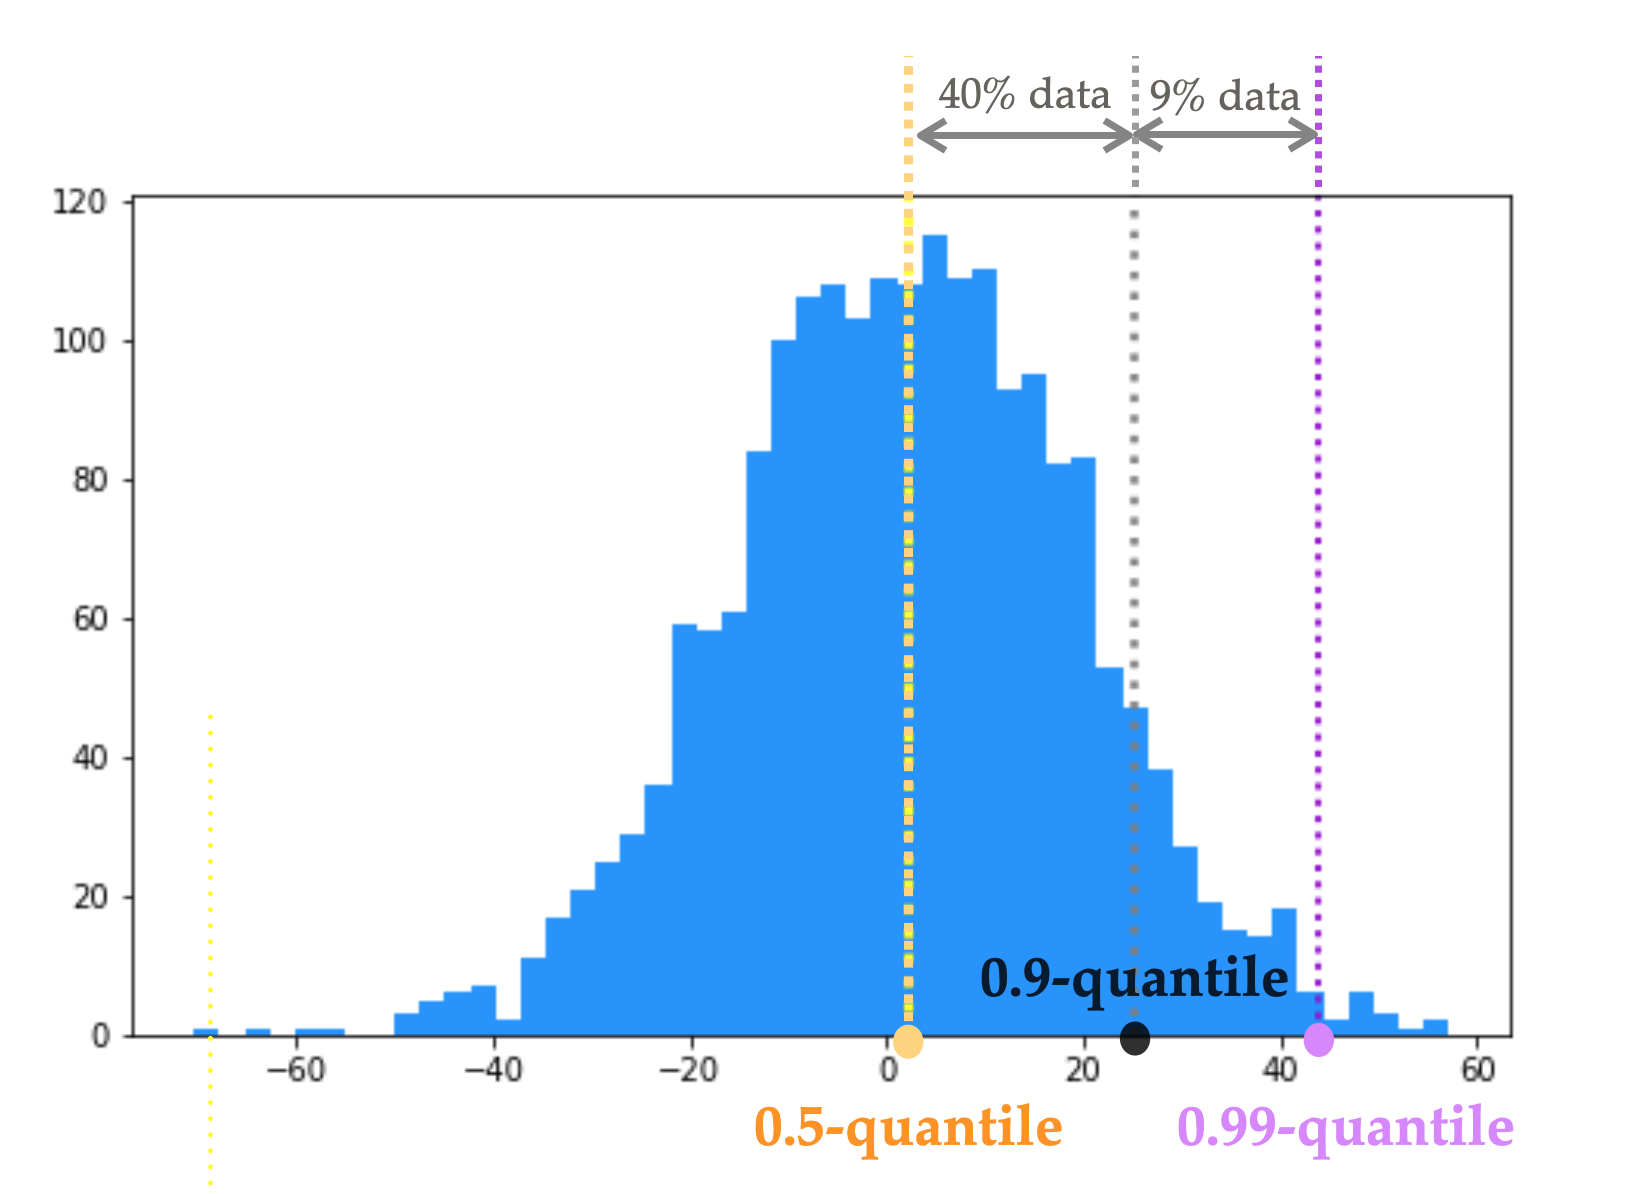
\includegraphics[width=0.6\columnwidth]{quant_example.png}
    \caption{Quantiles (0.5-q, 0.9-q and 0.99-q) of a dataset containing 2000 random samples from a Gaussian distribution (mean = 2, standard deviation = 18)}
    \label{fig: quant_example}
\end{figure*}

As shown in the example of Fig \ref{fig: quant_example}, the concept of quantiles are also applied in datasets as well as probability distributions. Similarly, the quantile for a finite dataset is the point which divides the dataset by probability $\tau$. However, since the dataset is discrete, the value of a $\tau$-q is ambiguous. For example, for dataset [$1,2,3,4$], both 2.01 and 2.99 can be considered as a valid value of $0.5$-q. Among various methods of dataset quantile estimations, we apply the one currently used by the \textit{Python 3} language. For a size $N$ dataset $X = \{x_1, ..., x_N\}$ , the method first finds the ranking index of the quantile $h = (N-1)\tau + 1$. If $h$ is not an integer, the estimated quantile is computed by linear interpolation between the two data points at ranking positions surround $h$
\begin{equation}
    \tau \text{-q}_{batch} = x_{\lfloor h\rfloor}+(h-\lfloor h\rfloor)\left(x_{\lfloor h\rfloor+1}-x_{\lfloor h\rfloor}\right)
\end{equation}
where $\lfloor h\rfloor$ is the greatest integer less than or equal to $h$. The computation result $\tau \text{-q}_{batch}$ is called a \textit{batch quantile}, since it comes from a batch of samples of a distribution.
\\\\
Note that although computing the quantiles of a sample estimates the quantiles of the associated distribution, this is not \"quantile estimation\" as it is referred to in this paper. Here the batch quantiles are regarded as computed quantiles, as a comparison of \textit{true quantiles} which are the real quantiles of the original probability distribution. The estimation of quantiles is introduced in the following part.

% Batch algorithm/True quantile: the naive sorting

\section{Data streams and quantile estimation}
\label{sec: intro_quant_est}

A \textit{Data stream} is a large source of data where data is created in sequence over a period of time. In contrast with datasets, data points are not instantly available all at a time, and that the size of the sample grows over time. Data streams are commonly seen in areas like network monitoring, data mining, financial trading systems, etc. Similarly to normal datasets, the value of quantiles is important for data analysis of data streams. Finding the quantiles of a data stream is the initial aim of this paper.

A trivial solution to find quantiles of data streams is to sort the entire data stream when the last data point arrives, and then compute the batch quantiles of the sorted dataset.  In cases when the size of the data stream is unknown, at the arrival of each data point, the batch quantiles are computed again so the quantile values get updated. The method of repeatedly sorting and computing batch quantiles is called the \textit{batch algorithm}. Due to the large size of the data streams, the batch algorithm for quantile computation is too expensive in both storage and computation to be a feasible solution for most computer systems.

Faced with the storage and computation problem, algorithms of \textit{quantile estimation} on data streams have been proposed. The quantile estimation algorithms do not store the entire data streams, and the algorithms return estimated quantiles that are close to the batch quantiles. Some quantile estimation algorithms are described in the literature review chapter. Although these algorithms use significantly less memory than the batch algorithm, most require a growing space complexity (i.e., correlated with size $N$). In this paper we investigate the space-efficient algorithms that use constant memory units for data streams of any size. Specifically, we focus on the machine learning method \textit{stochastic gradient descent} (SGD) for quantile estimation. 

\section{Stochastic gradient descent(SGD) for quantile estimation}
\label{sec: intro_GD_SGD}

\textit{Gradient descent} is a convex optimization algorithm that is commonly used in machine learning for loss function minimization. Gradient descent takes the entire dataset as the input, and by iteratively moving in the opposite direction of the gradient, it reaches the local minimum. Such method can also be used in quantile estimation if the entire dataset is available all at the same time.

\textit{Stochastic gradient descent (SGD)}, on the other hand, is the "online learning" version of gradient descent that updates iteratively when each new data point comes. For each data point, SGD steps in the opposite direction of the gradient computed from that data point. In this way, SGD updates using one data point at a time, rather than the whole dataset.
Fig \ref{fig: SGD_quant} shows how SGD is used to estimate quantiles on the same dataset of 2000 Gaussian distribution samples from Fig 1. It is shown in the figure that the SGD result fluctuates around the empirical quantile value, indicating SGD is a possible approach for quantile estimation.

\begin{figure*}[h!]
    % \centering
	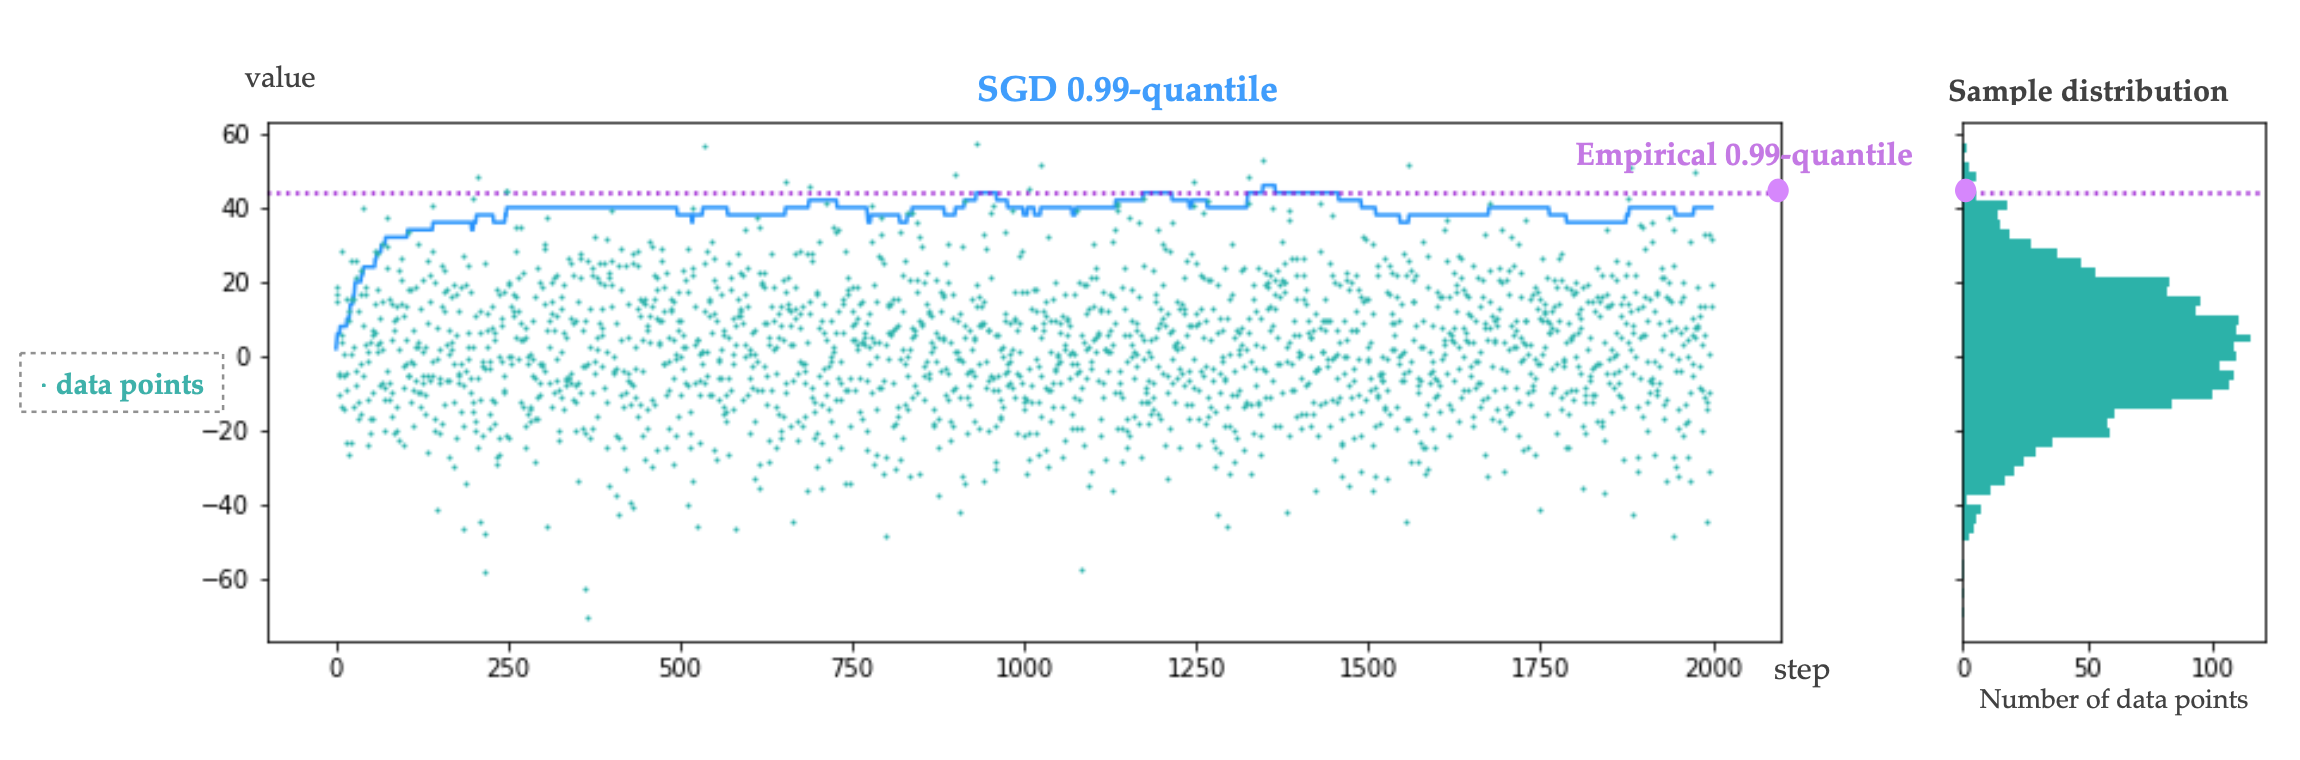
\includegraphics[width=1\columnwidth]{SGD_gaussian.png}
    \caption{SGD quantile estimation of the $0.99$-q for a dataset of 2000 samples from a Gaussian distribution. The left graph is a combination of incoming data points and the SGD steps, and each step of SGD is triggered by a new coming data point. The blue line shows how the SGD result is updated on the arrival of a data point (sea-green), and straight line (violet) represents the empirical value of $0.99$-q. On the right side, the density of the bell-shaped dataset is shown in a histogram.}
    \label{fig: SGD_quant}
\end{figure*}


\section{Background}

In this chapter, the essential background knowledge assumed throughout the rest of this thesis is defined. Subsection~\ref{subsec: sgd}introduces Stochastic Gradient Descent (SGD), which is a convex optimisation approach commonly found in machine learning, and subsection~\ref{subsec: quant} provides a definition for quantiles.
Stochastic gradient descent (SGD) is a convex optimization approach commonly applied in machine learning, and quantiles are the dividing points of a distribution or a dataset.

    \subsection{Gradient descent and stochastic gradient descent}
    \label{subsec: sgd}
    Stochastic gradient descent is an optimization algorithm developed from gradient descent. 
    % \marginpar{References to be added here}
    % Gradient descent was introduced by \textcolor{blue}{someone}, and is commonly used in \textcolor{blue}{something}

    \subsubsection{Gradient Descent}
        For convex optimization problems, gradient descent is a first-order optimization algorithm 
        to find the local minimum of a function.
        \\\\
        To solve the minimization problem 
        \begin{equation}
            % E
            \min_{\x} L(\x) 
        \end{equation} 
        
        where $L : \R^d \to \R$ is convex, differentiable and its gradient is Lipschitz continuous with constant
        $L > 0$.
        \\\\
        Geometrically, the gradient $\nabla L(\x_0)$ points to the direction of the steepest ascent on $L(\cdot)$ 
        from the point $\x_0$. 
        By taking a small step in the direction of the negative gradient, the function value is decreased in the 
        direction of the steepest descent. That is,
        \begin{equation}
            \x_1  = \x_0 - \alpha \nabla L(\x_0)
        \end{equation}
        for a small enough step size $\alpha \in \R_{+}$, then $L(\x_1) \leq L(\x_0)$. 
        That means, compared with $L(\x_0)$, $L(\x_1)$ is closer to the local minimum.
        \\\\
        With this observation comes the idea of gradient descent: an iterative "tour" on $L(\cdot)$ from a point towards the 
        local minimum by following small steps of negative gradient. 
        Let $\x_0$ be the guess of a starting point, then if
        % \marginpar{notation k should be i}
        \begin{equation}
            \x_{i+1} = \x_{i} - \alpha_i \nabla L(\x_i), i \geq 0
        \end{equation}
        
        
        Then we have $ L(\x_0) \geq L(\x_1) \geq L(\x_2) \geq \cdots$ where $\alpha_i$ is a suitable step size for iteration $i$. The convergence rate of the 
        sequence $(\x_n)$ with certain step size settings is linear in terms of the number of iterations.

        The objective function $L(\cdot)$ can be written as a sum of differentiable functions:%
        \begin{equation}
            L(\x) =\frac{1}{N} \sum_{n=1}^{N} \ell_n (\x)
        \end{equation}

        where the \textit{summand function} $\ell_n$ is usually the loss function of the $n$th observation among
        $N$ data points.
        \\\\
        Applying the gradient descent formula, $\x$ is updated according to%
        %
        \begin{equation}
           \x_{i+1} = \x_{i} -\alpha_i \nabla L(\x_i) = \x_{i} -\alpha_i \frac{1}{N}\sum_{n=1}^{N} \nabla \ell_n(\x_i) 
           \label{eq: background_gd_summand}
        \end{equation}

        From formula~\ref{eq: background_gd_summand}, it is clear that gradient descent requires access to all the data points to compute the movement direction, which is infeasible for a data stream.


    \subsubsection{Stochastic Gradient Descent (SGD)}
        % Stochastic gradient descent was \textcolor{blue}{introduced by who because blabla, and commonly used bla}
        It is the choice for data streams, because the computation of the movement direction relies only on the most recent data point.
        It can be considered as a stochastic approximation of gradient descent optimization.
        \\\\
        The calculation of $\sum_{n=1}^{N} \nabla \ell_n(\x_i)$ can be
        expensive, especially when the amount of summand functions is huge, or when the individual gradients are hard to
        compute.
        To reduce the calculation, an estimation of the true gradient of $L(\x)$ is taken: 
        the true gradient $\frac{1}{N} \sum_{n=1}^{N} \nabla \ell_n(\x_i)$ is replaced by the gradient with respect to the $m$th observation, $\nabla \ell_m(\x_i)$. 
        So the update of the parameter $\x$ becomes%
        \begin{equation}
            \x_{i+1} = \x_i - \alpha_i \nabla \ell_m(\x_i)
            \label{eq: intro_SGD}
        \end{equation}
        
        Generally, each time $m$ is randomly selected from $N$. In this paper, we use $m = i$ for quantile estimation on data streams.

\subsubsection{Limitations}
% \marginpar{Not sure how I should mention this non-differentiable issue}
Since each SGD update requires only a single data point instead of the entire dataset, it becomes a great alternative for quantile estimation.
However, neither GD nor SGD can handle non-differentiable functions. This is an issue for the quantile estimation loss function in the following chapter.
Furthermore, while the computation per update is decreased $N$ times, the tradeoff lies in the convergence rate. SGD does not enjoy the same linear convergence rate as gradient descent. Both of these issues are discussed in chapter~\ref{ch: stepsize_adaptation}.


\subsection{Quantile}
\label{subsec: quant}

In statistics, quantiles are the points that divide a probability distribution into even intervals.
The $q$-quantiles ($q \in \{2,3,4,...\}$) is a set of quantile points which divides the distribution into $q$ intervals each with the same probability mass.
For example, the $2$-quantile has only one quantile point, which is the middle point of the distribution
and it divides the distribution into two even parts. This $2$-quantile point is called the median.
        \\\\
    \textbf{Definition with $q$-quantile notation} \\
    Generally, the $q$-quantiles have $q-1$ quantile points, and the $k$th quantile point for a 
    distribution $X$ is the data value such that%
    %
    \begin{equation}
        Pr(X \leq x) \geq \frac{k}{q}
    \end{equation}
    
    and%
    %
    \begin{equation}
        Pr(X \geq x) \geq 1 - \frac{k}{q}
    \end{equation}
    where $x \in X$.
    \\\\
    \textbf{Definition with notation $\tau$}\\
    Since $k < q$, we have $0 < \frac{k}{q} < 1$ for all ($k$,$q$) pairs. For $k, q \in \mathbb{N}^+$ we can define a quantile for any rational number in the interval $(0,1)$. For a quantile probability $\tau$, we use the notation $\tau$-quantile ($0 < \tau < 1$) for a quantile value in the distribution $X$ that satisfies%
    %
    \begin{equation}
        Pr(X \leq x) \geq \tau
    \end{equation}
    
    and%
    %
    \begin{equation}
        Pr(X \geq x) \geq 1 - \tau
    \end{equation}
    where $x \in X$.



\section{Thesis overview}
\label{sec: intro_overview}

This thesis aims to thoroughly answer the following question:
\begin{quote}
\emph{Can SGD be used for effective quantile estimation?}
\end{quote}

In investigating the above research question, this thesis includes the following contributions:
\begin{enumerate}
    \item Proposal of the SGD algorithm for quantile estimation which implements the SGD approach.
    \item SGD algorithm performance comparison with the state-of-the-art Frugal1U.
    \item Identification of some contributing factors on SGD performance.
    \item Improved SGD methods with quicker convergence rate to the true quantile value.
    % \marginpar{This is not counted as a contribution I think?}
    \item Experiments on other people's methods that simultaneously estimate different quantiles at the same time, which is a potential improvement direction for SGD too.
\end{enumerate}

In the final part of the introduction, we give a brief tour of the material in this paper. The main focus of the paper is to explore how stochastic gradient descent method can be used for quantile estimation on data streams.
In chapter \ref{ch: literature_review}, a very brief discussion of quantile estimation algorithms is presented, with a special mention for space-efficient algorithms (e.g., SGD-like methods). 
Chapter \ref{ch: algo_equal} compares the SGD methods with the \textit{Frugal1U} algorithm\cite{maFrugalStreamingEstimating2014}, showing how the two similar methods are "equivalent" to some extent.
Chapter \ref{ch: sgd_exp} which presents experiments to illustrate the relationship between setting for SGD and its performance.
Next, chapter \ref{ch: stepsize_adaptation} and \ref{ch: multi_quant} explore the two extensions of the vanilla SGD algorithm: the step size adaptation of SGD and the simultaneous multi-quantile estimation. Finally, the work of the paper is summed up in the conclusion chapter \ref{ch: conclusion}.
\\\\
Fig \ref{fig: structure} is the layout of the contents of the paper.

\begin{figure*}[h!]
    \centering
	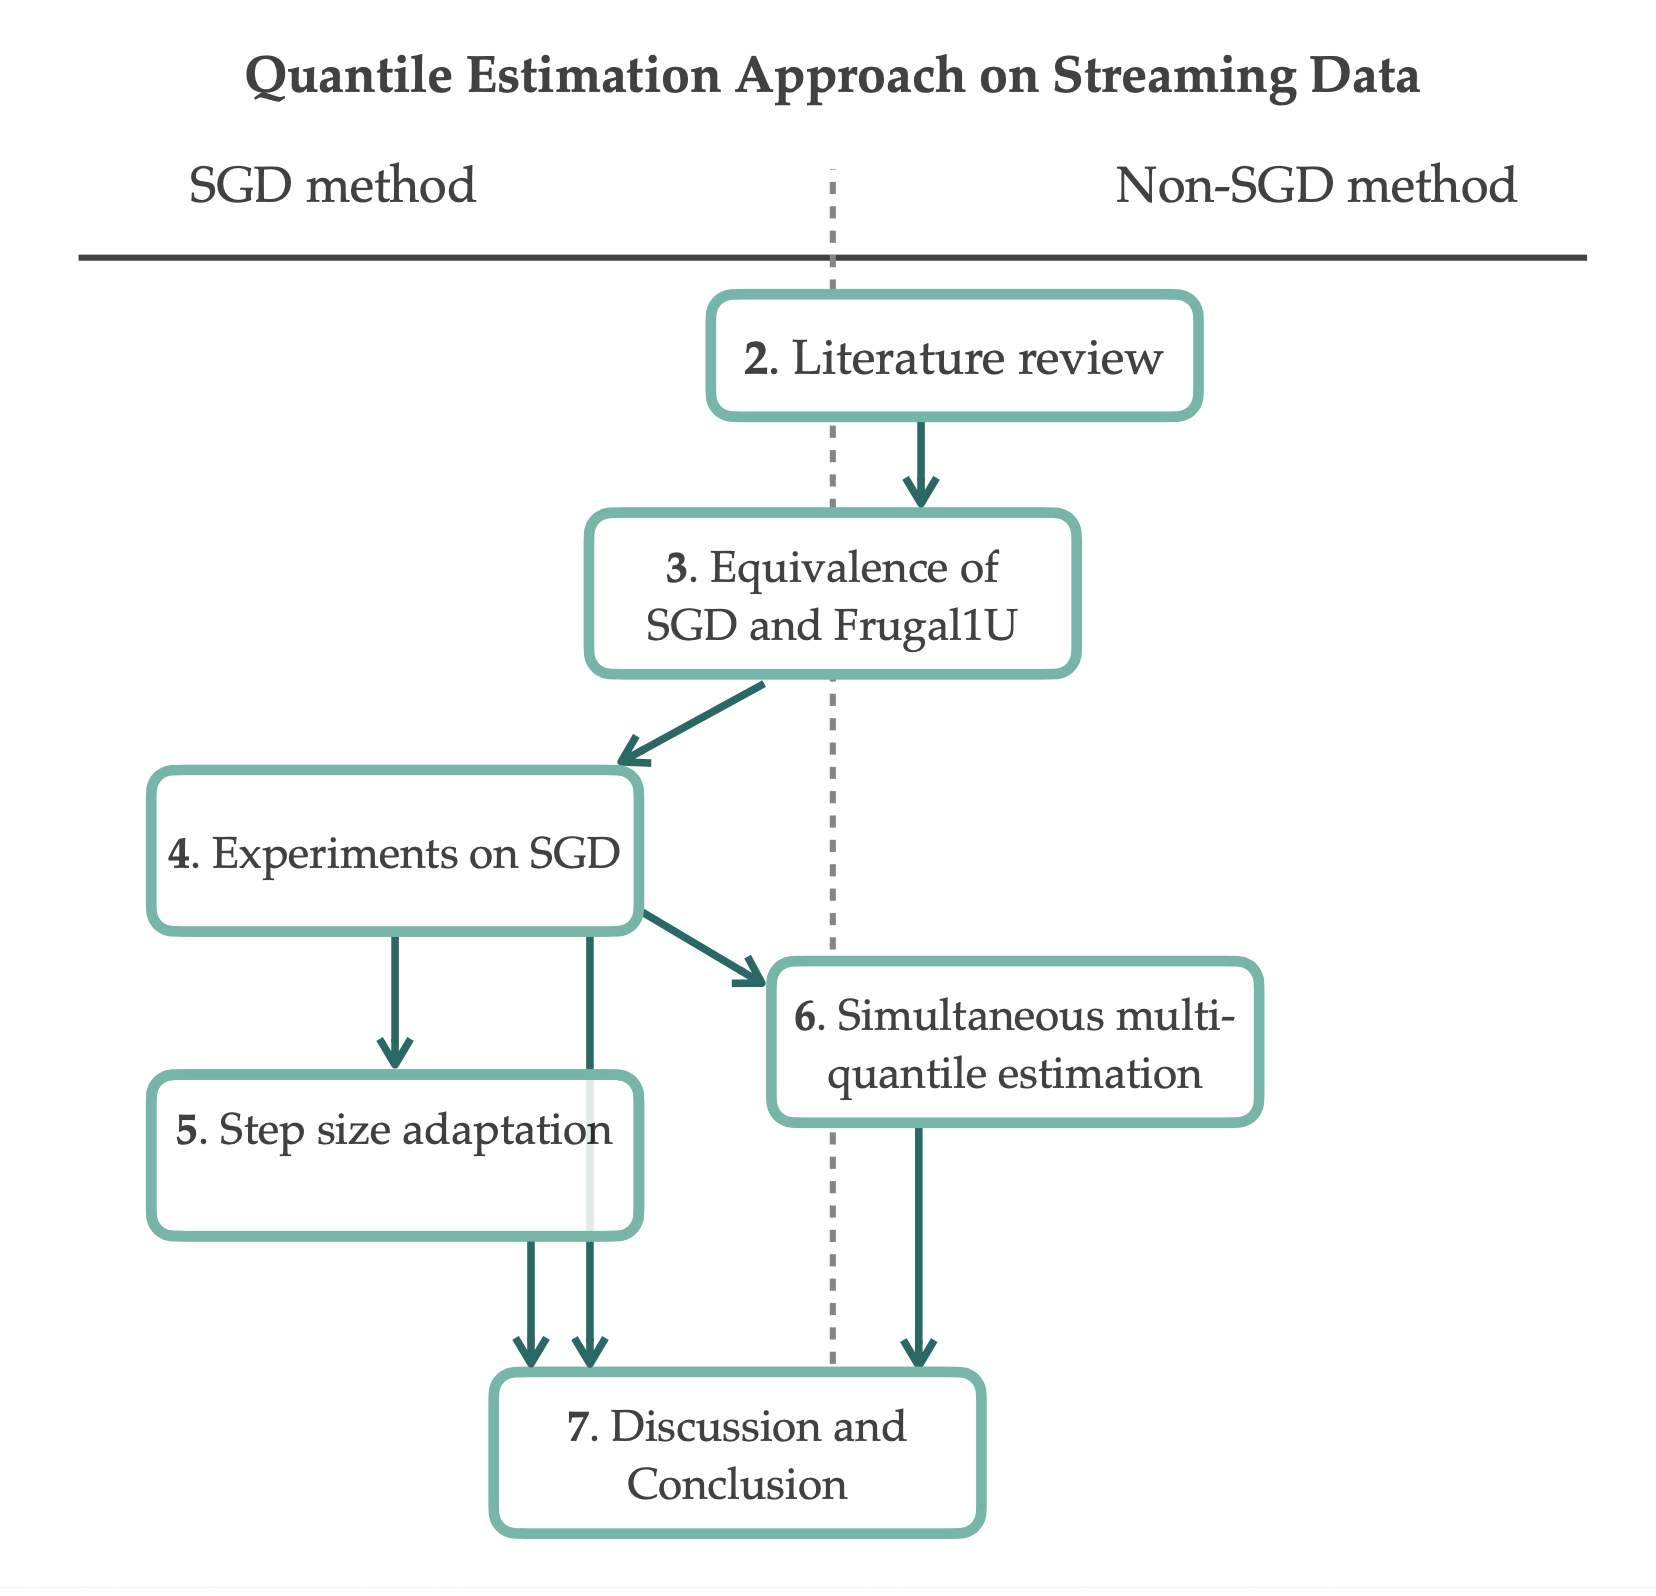
\includegraphics[width=0.8\columnwidth]{structure.png}
    \caption{The relationship between topics covered in the thesis. Topics are roughly positioned along the top-bottom axis depending on where they are more close to SGD methods (left) or non-SGD methods (right). The arrows between the chapters represent are connected according to dependence.}
    \label{fig: structure}
\end{figure*}

% \marginpar{My contributions to be added here}
\documentclass[12pt]{article}
\usepackage{xcolor}
\def\R{\rm I\!R}
\def\x{\bm{x}}
\usepackage[numbers]{natbib}

\title{Literature review outline}
\date{\vspace{-5ex}}


\begin{document}
\maketitle

\section{SGD 
            \color{blue}{(should it be in Background instead?)}}
    

\section{Quantile Estimation From Streaming Data}
\begin{enumerate}
    \item Why useful: \\
        \cite{rayArtApproximatingDistributions1800}(Industrial use) "
        Many businesses care about accurately computing quantiles over their key metrics, which can pose several interesting challenges at scale. 

        e.g. Price for advertisement on bidding level: quantile estimation helps price setting
        "\\\\
        Other industrial usage mentioned in \cite{hongEstimatingQuantileSensitivities2009}, and its citations for industrial use \\
        "
        Quantiles have been adopted by many industries as major
        measures of random performance. In the financial industry,
        quantiles, also known as value-at-risks (VaRs), are widely
        accepted measures of capital adequacy. For example, the
        Bank for International Settlement uses the 10-day VaR at
        the 99\% level to measure the adequacy of bank capital
        (Duffie and Pan 1997). In the service industry, quantiles
        are often used as measures of service quality. For example, the service quality of an out-of-hospital system is frequently measured by the 90th percentile of the times taken
        to respond to emergency requests and to transport patients
        to a hospital (Austin and Schull 2003). Quantiles have
        also been used as billing measures in some circumstances.
        For example, some Internet service providers (ISPs) charge
        their users based on the 95th percentile of the traffic load
        in a billing cycle (Goldenberg et al. 2004).
        "
    % \item Pinball loss on quantile regression: \\
    %     \cite{steinwartEstimatingConditionalQuantiles2011}\\
    %     \cite{koenkerRegressionQuantiles1978}
    % \item Simultaneously predicting several quantiles: \\
    %     \cite{sangnierJointQuantileRegression} (non-streaming)(multi-dimensional)(quantile regression)\\
    \item Quantile Streaming: \\
        \cite{greenwaldQuantilesEquidepthHistograms2016}\\
        They propose a property on quantile estimation which guarantees accuracy within a pre-specified precision. 
        \textbf{$\epsilon$-approximate $\phi$-quantile}
        It is good(????) for algorithms with equidepth histogram method.
        A new algorithm for $\epsilon$-approximate quantiles with space complexity $O(log(\epsilon n)/\epsilon)$ is proposed. It is inspired by \textbf{Manku, Rajagopalan}'s work. 
         The problem is, the memory passes into the device(???) is affected by data size.
        \\\\
        \cite{maFrugalStreamingEstimating2014}\\
    \pagebreak    
    \item Parallel estimation \textbf{on other things} from Streaming Data: \\
        % \cite{jainP2AlgorithmDynamic1985}\\
        Related work on parallel quantile estimation on streaming data.



        Multiple quantile estimation from streaming data requires the estimation of several different quantile values being calculated simultaneously from streaming data. It has been an issue targeted by different algorithms.\\\\

        \cite{ben-haimStreamingParallelDecision} 
        \textbf{A Streaming Parallel Decision Tree Algorithm}

        The Streaming Parallel Decision Tree (SPDT) algorithm \cite{ben-haimStreamingParallelDecision} introduces an on-line histogram building method % from streaming data at parallel processors.
        in which histogram boundaries are estimated quantile values.
        In this method, multiple histograms are built from streaming data in parallel, which are then merged into a summary histogram of the entire dataset. The summary histogram is a set of sorted real numbers that represents the interval boundaries such that all the intervals have approximately the same size. Specifically, for a summary histogram with $N$ intervals, the set of real numbers is approximately the set of $\tau$-quantiles ($\tau = \frac{1}{N}, \frac{2}{N}, ..., \frac{N-1}{N}$) for the input data stream.

        This method works for distributed system where big data stream is processed by different processors. It also works well for huge amount of data because the computation complexity is not affected by the size of dataset.
        % This summary histogram is notable for its evenly distributed intervals sizes, as each interval has the same number of data points. To interpret the histogram into quantiles, 
        \\\\
        \cite{pebayFormulasRobustOnepass2008}\\

\end{enumerate}

\section{Anomaly Detection and Outlier}

\begin{enumerate}
    \item Anomaly detection: \\
        \cite{emmottMetaAnalysisAnomalyDetection2015}
        (industrial use)
        ()
        % \cite{huangOnlineAnomalousTime2013}
\end{enumerate}
\newpage
\textbf{My work} Quantile estimation on streaming data, which would be applied on 

\newpage
% \citeauthor{blassWhenAreTwo2008}
\bibliography{Thesis}
\bibliographystyle{IEEEtranN}

\end{document}
\end(documentclass) % Chapter 2
\documentclass[11pt]{article}

\def\R{\rm I\!R}
\def\x{\bm{x}}

\title{Proof of Algorithm Equivalence}
\author{Yiping Su}
\begin{document}
\maketitle
% --------------------------------------------------------------------------------
%                                Quantile Estimation
% --------------------------------------------------------------------------------
            
\section{Quantile Estimation}

\subsection{Quantile}

In statistics, quantiles are the points that divide a probability distribution into even intervals.
The $q$-quantiles devide the distribution into $q$ intervals each with the same amount of data points.
And there are $q$ quantile points of the $q-$quantiles.
For example, the $2$-quantile has only one quantile point, which is the middle point of the distribution
and it divides the distribution into two even parts. This $2$-quantile point is called the median.


\subsubsection{Definition} \label{tau-quantile-def}
Generally, the $q$-quantiles have $q-1$ quantile points, and the $k$th $q$-quantile for a 
distribution $X$ is the data value such that
$$
Pr(X \leq x) \geq \frac{k}{q}
$$
and
$$
Pr(X \geq x) \geq 1 - \frac{k}{q}
$$
where $x \in X$

\subsection{Quantile Estimation and Pinball Loss}
In this paper, the estimation for $\tau$-quantile 
($\tau =  \frac{1}{q}, \frac{2}{q}, \cdots, \frac{q-1}{q}$)
is applied.
Pinball loss function is one of the approaches for the estimation for a statistical population.
\\\\
For a one-dimentional data set $X = \{x_1, x_2, \cdots, x_N\}$, 
now consider the loss function for a single data point $x$ $(i \in {1, \cdots, N})$.
Let $t := x - q$ be the difference between the real value $x$ and the estimate of quantile $q$.
$l_{\tau}(\cdot): \R \to \R_{\geq 0}$ is the loss function on $t$ such that
$$
l_\tau(t)= 
    \begin{cases}
        \tau t & t > 0\\
        -(1-\tau) t & otherwise
    \end{cases}
$$
And the $\tau$-quantile loss has the {\color{red} subgradient}:
$$
\frac {\partial l_\tau(t)}{\partial t}= 
    \begin{cases}
        \tau                & t > 0\\
        -(1-\tau)           & t < 0\\
        [\tau, -(1 - \tau)] & t = 0
    \end{cases}
$$

The overall loss for distribution $X$ with quantile estimation $q$ is
$$
L_{\tau}(q) = \sum_{x \in X} l_{\tau}(x - q)
$$
The best estimate of the $\tau$-quantile $q$ is the $q$ with minimal overall loss. 
Let $q^\ast$ be the best estimate, then we have
$$
q^\ast = \argmin_{q} L_{\tau}(q)
$$


% --------------------------------------------------------------------------------
%                                SGD for Quantile Estimation
% --------------------------------------------------------------------------------
\section{Algorithm Equivalence}

\subsection{Pseudo Code for the Frugal-1U Algorithm}

Qiang Ma, S. Muthukrishnan and Mark Sandler {\color{red} [ref]}  
introduced the following algorithm \ref{alg:frugal_1U} which 
"uses only one unit of memory per group to compute a quantile for each group"({\color{blue} quotation}).

\begin{algorithm}
\caption{Frugal-1U}\label{alg:frugal_1U}
    \begin{algorithmic}[1]
        \Require{Data Stream $S$, $h$, $k$, $1$ unit of memory $\tilde{m}$}
        \Ensure{$\tilde{m}$}
        % \Procedure{frugal}{$X,\tau$}            \Comment{X is the dataset}
        \State {Initialization $\tilde{m} = 0$}               %\Comment{Default initialization $q_0$ = 0}
            \For{\textbf{each} $s_i$ in $S$}                  %\Comment{Parameter update for each input data point}
                \State{$rand$ = random(0,1); //get a random value in $[0,1]$}
                % \State {\textbf{set} $\alpha_k$} \Comment{Set stepsize}
                \If{$s_i > \tilde{m}$ \textbf{and} $rand > 1-\frac{h}{k}$} %\Comment{$q_{k+1} = q_k + \alpha_k \tau$ when $x_k - q_k > 0$}
                    \State{$\tilde{m} = \tilde{m} + 1$;}
                \Else { \textbf{if} $s_i < \tilde{m}$ \textbf{and} $rand > \frac{h}{k}$}  %\Comment{$q_{k+1} = q_k - \alpha_k (1-\tau)$ otherwise}
                    \State{$\tilde{m} = \tilde{m} - 1$;}
                \EndIf
            \State{\textbf{end if}}
            \EndFor
        \State{\textbf{end for}}
        % \State \textbf{return} $q$              \Comment{$q_k$ is the SGD result of quantile estimate}
        % \EndProcedure
    \end{algorithmic}
\end{algorithm}
The output $\tilde{m}$ is the estimate of the $h$th $k$-quantile for a given data stream $S$. 
By rephrasing of some steps of Frugal-1U, 
its equilalence to an SGD algorithm for quantile estimation will be shown in the follwing part.
\\\\
\textbf{Rephrasing of the Algorithm} \label{replacements}
\begin{enumerate}
    \item The constant $\frac{h}{k}$ is replaced by $\tau$, since the $\tau$-quantile is defined
     as the $h$th $k$-quantile point in section \ref{tau-quantile-def}.
    % \item The quantile estimate $\tilde{m}$ is replaced by $q$, as it stands for estimate of quantile.
    \item The generation of random number and it's comparison with $1-\frac{h}{k}$ or $\frac{h}{k}$
    in line 3 to 7 is replaced by the following algorithm.
    \begin{algorithm}
        \begin{algorithmic}[1]
            \setcounter{ALG@line}{2}
            \State{ }   \Comment{No need to generate a random number}
            \If{$s_i > \tilde{m}$} %\Comment{$q_{k+1} = q_k + \alpha_k \tau$ when $x_k - q_k > 0$}
                \State{$\tilde{m} = \tilde{m} + 1 \times (1-\frac{h}{k})$}     
                \Comment{$P((rand > 1-\frac{h}{k}) \mid rand \in \mathcal{U}(0,1)) = 1-\frac{h}{k}$;}
            \Else { \textbf{if} $s_i < \tilde{m}$}  %\Comment{$q_{k+1} = q_k - \alpha_k (1-\tau)$ otherwise}
                \State{$\tilde{m} = \tilde{m} - 1 \times \frac{h}{k}$}         
                \Comment{$P((rand > \frac{h}{k}) \mid rand \in \mathcal{U}(0,1)) = \frac{h}{k}$;}
            \EndIf 
        \end{algorithmic}
    \end{algorithm}

    % Here the probability $P((rand > p) \mid rand \in \mathcal{U}(0,1))$ is the simplification
    % for the generation of random number $rand$ and it's comparison to a constant $p$ $(0 < p < 1)$.
    
    To understand this replacement, let's consider the serie of the 3 steps: 
    (i) generate a random number $rand$, 
    (ii) compare it with a constant $p$, and
    (iii) take action if $rand > p$. 
    It can be interpreted as take the action with probability 
    $P((rand > p) \mid rand \in \mathcal{U}(0,1))$. 

    Mathmatically, the replacement works because the expected change of
    $\tilde{m}$ in both methods are the same. 
    For example when $s_i > \tilde{m}$, 
    the expected change of $\tilde{m}$ is
    $E_1[\nabla \tilde{m}] = E[\tilde{m} \times p]$ in the Frugal-1U with 
    random number generation,
    while 
    $E_2[\nabla \tilde{m}] = \tilde{m} \times p$ in the replacement method.
    Since $E_1[\nabla \tilde{m}] = E_2[\nabla \tilde{m}]$, the replacement is valid
    with regard to the expectation of the change in quantile estimate during each step.

\end{enumerate}


\subsection{SGD for Loss function}

Let $q_0$ be the initial guess of quantile estimate. 
By SGD, the estimate is updated each step with a data point from the distribution.
$$
q_{k+1} = q_k - \alpha_k g_k
$$
where $ \alpha_k $ is a suitable stepsize and 
$$
g_k = \partial L_{\tau}^{(k)}(q_k) \in \frac{\partial l_\tau(x_k - q_k)}{\partial q_k}
$$ 
\textbf{Notice: partial is taken because the gradient of a single variable function
euqals the partial of it}
\\\\
Then we have
$$
q_{k+1} = 
    \begin{cases}
        q_k + \alpha_k \tau               & x_k - q_k > 0\\
        q_k - \alpha_k (1-\tau)           & x_k - q_k \leq 0\\
        % [\tau, -(1 - \tau)] & t = 0
    \end{cases}
$$

\begin{algorithm}
    \caption{SGD algorithm}\label{alg:SGD}
    \begin{algorithmic}[1]
        \Require{Data Stream $X$, $\tau$, $1$ unit of memory $q$}
        \Ensure{$q$}
        % \Procedure{frugal}{$X,\tau$}            \Comment{X is the dataset}
        \State {Initialize} $q$                 \Comment{Default initialization $q_0$ = 0}
            \For{$x_k$ in $X$}                  \Comment{Parameter update for each input data point}
                \State \textbf{set} $\alpha_k$  \Comment{Set stepsize}
                \If{$x_k > q$}                  \Comment{$q_{k+1} = q_k + \alpha_k \tau$ when $x_k - q_k > 0$}
                    \State{$q = q + \alpha_k \tau$}
                \Else                           \Comment{$q_{k+1} = q_k - \alpha_k (1-\tau)$ otherwise}
                    \State{$q = q - \alpha_k (1-\tau)$}
                \EndIf
            \EndFor
        \State \textbf{return} $q$              \Comment{$q_k$ is the SGD result of quantile estimate}
        % \EndProcedure
    \end{algorithmic}
\end{algorithm}
% --------------------------------------------------------------------------------
%                              Equality of two algorithms 
% --------------------------------------------------------------------------------
\section{Equivalence of Algorithms}
In this section we'll show the equilalence of algorithm Frugal-1U 
and SGD.
\\\\
Besides the replacements mentioned in section \ref{replacements},
the notations have changed: 
$X$ is applied for the data stream, and $q$ instead of $\tilde{m}$
to represent quantile estimate.
The introduction of changable stepsize $\alpha_k$ for each data point $x_k$
is the highlight of the SGD algorithm. The flexibility of stepsize can help
with achieving a better convergence rate when stepsizes are chosen wisely.
Specifically, the setpsize is not mentioned in Frugal-1U 
because it is fixed as $1$. In SGD the stepsize might change for every step.

{\color{red} \textbf{Problem}}
In Frugal-1U the quantile estimate $q$ does not change when $x_k > q$, but in SGD 
the quantile estimate is updated: $q = q-\alpha_k (1-\tau)$. This can be seen as different 
\textbf{subgradient} values for $l_\tau(x_k - q_k)$ 
{\color{red} \textbf{but then I need to explain subgradient descent}} 


\end{document}


\documentclass[12pt]{article}
\usepackage{xcolor}
\usepackage[nointegrals]{wasysym}

\def\R{\rm I\!R}
\def\x{\bm{x}}

\title{SGD Quantile Estimation Experiement}
\date{\vspace{-5ex}}

\begin{document}
\maketitle

\section{Introduction}

% \subsection你说“我就不该这么想”{Aims}
This experiment has two purposes. The first is to show quantile estimation with SGD works \textcolor{blue}{ under some circimstances (?)}.
The second aim is to investigate how different settings of the problem effect the estimation performance. Specifically, we are interested in the following aspects: data distribution, data size, data ordering, quantile value and sgd step size.
In the experiment, multiple ordered datasets are generated as input data streams, based on which the calculated and estimated quantile values are computed. Results of both quantiles are compared after processing. We want to compare the performance of quantile estimation over different settings.
\\\\
\textcolor{blue}{This experiment also aims at the comparison between Frugal algorithm and SGD algorithm, by which we want to show that those two algorithms are ``equivalent". 
\\
(Does it mean SGD estimation works?)}
% To test the SGD quantile estimation as a valid alternative for quantile estimation, this experiment computes both estimated and calculated values for quantiles, and evaluates whether the difference between the results is acceptable.
% \\\\
% Do I explain the second goal...?


\section{Methodology}
The process by which we experiment on SGD quantile estimation can be briefly outlined as followes:

\begin{enumerate}
    \item Select a set of data streams (ordered datasets) derived from some statistical distributions.
    \item For each $\tau$-quantile, determine a ground truth value from the distribution and calculate a empirical value from the data stream.
    \item For each $\tau$-quantile, calculate the SGD estimate value from the data stream, record both the process and the result of estimation.
    \item \textcolor{blue}{
        Compare Frugal algorithm and SGD algorithm on data streams of the same setting.
    }
    \item Compute normalized error value for quantile estimates as a measurement of similarity between empirical and estimate value. The error value is computed from both values.
\end{enumerate}

\subsection{Data Stream Set Generation}
A total of 4 distributions are used in this experiment.
Eah data stream is a set of 1 dimensional data points randomly sampled from one of the distributions. In order to show how the amount of data points might affect the performance, there are 3 different settings for the data size $N$. 
\\\\
Each data stream set is composed of a number of data streams. For a statistically more accurate results on the experiment, a group of data streams of the same settings are generated. When investigating the impact of data sequence has on quantile estimation, one data stream will be shuffled to for the generation to differently ordered data steams. To sum up, a data stream set is either a combination of data streams generated from same distribution and data size setting, or the permutations of one same data stream. We generate the data stream set under this settings:

\begin{itemize}
    \item Distribution: 4 statistical distributions. The 4 distributions are:
        \begin{itemize}
            \item Gaussian distribution 1: mean = 2, standard deviation = 18
            \item Gaussian distribution 2: mean = 0, standard deviation = 0.001
            \item Exponetial distribution: rate = 1
            \item Mixed Gaussian distribution: a mix of five different gaussian distributions
        \end{itemize}
    \item Data size: 100, 1000, 10000, 100000(?)
    \item Multiple generations: True or false. Generate 10 data streams for the set if true.
    \item Multiple shuffles:  True or false. Shuffle the data stream 10 times for the set if true.
\end{itemize}

\subsection{True and Empirical Quantile Calculation}
The true quantile values are the quantile values for the distributions which the data streams are derived from. They are calculated by the maths functions for quantile computation. All except the mixed gaussian distribution has a relatively easy function for quantile calculation. For the mixed distribution, the empirical quantile value from a large amount of sampling is taken for the true value. By this means, the empirical value is expected to be close enough to the true quantile value such that the evaluation of results is not much affected \textcolor{blue}{(needs more justification?)}. In this experiment, a total of 100,000,000 samples are generated for the calculation. For a certain $\tau$, there is only one true quantile value for one distribution.
\\\\
The empirical quantile value is the quantile value calculated from the data steam instead of the distribution. For a certain $\tau$, no matter what the ordering is, there is only one empirical quantile value for one data stream, but there can be multiple quantile values for one distribution.

\subsection{SGD Quantile Estimation}

The parameter of SGD quantile estimation is important. The current settings for step size $\alpha_k$ are:
\begin{itemize}
    \item Constant number: $\alpha_k =1$
    \item Decrease when k increases: $\alpha_k = \frac{2}{\sqrt{k}}$
    \item Decrease when k increases (smaller size): $\alpha_k = \frac{0.002}{\sqrt{k}}$
\end{itemize}
where $k$ is the index of step count.
\subsection{Frugal and SGD algorithm}

Frugal algorithm is proposed for quantile estimation as well. In this experiment, we want to compare the two algorithms and show they have similar performance for same data streams. In this experiment, data streams are generated from all 4 distributions, and the step size for SGD quantile estimation is set to constant 1.

\subsection{Error Computation}

An error measurement is proposed in order to evaluate the performance of quantile estimation. The error value represents the difference between empirical and estimated quantile value. For one data stream, the error function for its $\tau$-quantile is first defined as $E^{(\tau)} = | q_{batch}^{(\tau)} - q_{sgd}^{(\tau)} |$, where $E^{(\tau)}$ stands for the error, $q_{batch}^{(\tau)}$ for empirical quantile value and $q_{sgd}^{(\tau)}$ for SGD estimate value. For a specific data stream, a smaller $E^{(\tau)}$ means the estimation for the $\tau$-quantile has a better accuracy. Generally, for $n$ data streams of same size and distribution, we take the mean of the error value $\overline{E^{(\tau)}}$, where 
    $$
        \overline{E^{(\tau)}} = \frac{1}{n}\sum_{i=1}^{n} E^{(\tau)}_{i}
    $$
where $E^{(\tau)}_{i}$ is the error value of $\tau$-quantile for the $i$th data stream. To compare the performance of different settings of SGD estimation, we can now compare the $\overline{E^{(\tau)}}$ value for each setting.
\\\\
 Despite the capability of accuracy comparison, there is still room for improvement for this preliminary error measurement. 
% distribution
 First, the limitation of data distribution. The comparison is only available for data streams generated from the same distribution, since a different distribution has difference density of data points for the same $\tau$ value, leading to a failure of error comparison. For example, a data stream generated from uniform distribution $\mathcal{U}(0,1)$, the error value $\overline{E^{(0.1)}} = 2$ is a bad estimation, because 2 is even greater than the difference between the minimal and maximal value of the distribution ($2 > |0-1|$). However, for a data stream sampled from uniform distribution $\mathcal{U}(0,10^{10})$, $\overline{E^{(0.1)}} = 2$ might be a really accurate result, given how low the density is around its 0.1-quantile. 
% tau
 Second, the limitation of $\tau$ value. Similarly with the distribution problem, different $\tau$ values in the same distribution may have varied density. For example, for a gaussian distribution, $\overline{E^{(0.01)}} = \overline{E^{(0.5)}}$ means that the estimation is better for 0.01-quantile than 0.5-quantile, since the distribution is denser around the middle than its outlier.
% how it works
 Third and more importantly, it is incapable of showing if the estimation "works". Specifically, for some number $x$, we cannot find a reasonable explanation for the statement ``the estimate is accurate enough because we have $\overline{E^{(\tau)}} \leq x$''. Since for any $x$, we could find an example from the first two issues as a counter example. To solve those problems, a more general comparison of accuracy should be enabled by the new error measurement.
\\\\
In the new version of error value calculation, true quantile value of a data distribution $q_{true}^{(\tau)}$ is involved, so that $E^{(\tau)}$ is normalized by $|q_{batch}^{(\tau)} - q_{true}^{(\tau)}|$. It is now defined as
$$
    E^{(\tau)} = \frac{|q_{batch}^{(\tau)} - q_{sgd}^{(\tau)}|}
                      {|q_{batch}^{(\tau)} - q_{true}^{(\tau)}|}
$$
So that the accuracy of $q_{sgd}^{(\tau)}$ is compared with the accuracy of $q_{batch}^{(\tau)}$. The above problem is solved because \textcolor{orange}{to be continued}

\section{Observations}


\section{Discussion? Accuracy of study?}
% \begin{equation}
%     E = | \frac{q_{batch} - q_{sgd}}{{q_{batch}}^{(1)} - {q_{batch}}^{(2)}} |
% \end{equation}
\section{Conclusion}

\end{document}
\end(documentclass)
\chapter{Step Size Adaptation}
\label{ch: stepsize_adaptation}

\graphicspath{{Figures/Stepsize_adapt/}{./}} 

Step size is a key factor in convergence performance. The importance of step size selection is not only shown in our practical experiment results (chapter~\ref{ch: sgd_exp}), but has also been proved in theories of the machine learning ares. Generally in SGD, a large step size is likely to converge quickly and then have a high fluctuation rate. In contrast, a small step size can reduce fluctuation after it eventually converges, but the data stream might stop before convergence is reached.
Due to the fact that a small step size for one data stream might be a big one for another, we want to choose step sizes based on different measurements and heuristics. That is, we want to explore the topic of step size adaptation. 

In this chapter, we conduct an investigation of step size adaptation for SGD quantile estimation. Specifically, we look into two potential machine learning methods on step size adaptation, make analysis and implement one of them on SGD. In addition, we propose another step size adaptation algorithm, and compare the difference between their empirical performances. The contents of this chapther is listed as follows:

Section~\ref{sec: newton} briefly introduces the potential step size adaptation method in machine learning, and explains why it cannot be applied for the SGD algorithm.

Section~\ref{sec: sag} analyses another machine learning method \textit{SAG}, implements it to SGD and conducts experiments to check the convergence performance

Section~\ref{sec: DH_SGD} shows a proposal of another step size adaptation algorithm \textit{DB-SGD}, which is also provided with explanations and empirical experiments.

Section~\ref{sec: stepsize_adaptation_conclusion} compares the two proposed algorithms and discusses about their improvements on convergence.

\section{Failure on Newton's Method}
\label{sec: newton}
Newton's method is an iterative method to find the stationary points (where the function's derivative is zero) of a twice-differentiable function $f$. The application of Newton's method failed for our SGD quantile methods, since the loss function of the quantile estimation function is not twice-differentiable. For a specific $\tau$, let $t := x - q$ be the difference between the input data value $x$ and the estimate of quantile $q$, the loss function 

\begin{equation}
    \ell_\tau(t)= 
        \begin{cases}
            \tau t & t > 0\\
            -(1-\tau) t & otherwise
        \end{cases}
\end{equation}


is a linear function of $t$, which doesn't have any second derivative. 
\\\\
Though the method cannot be applied, it is easy to reach the goal of Newton's method: to find the critical points of a function. Instead of stationary point, the loss function has a critical point where it is not differentiable and the derivative changes sign. For any $\tau \in (0,1)$, when $t=0$, the loss function reaches it's critical points at $\ell_\tau(0) = 0$. Taking the critical point for each observation, however, does not contribute to any improvement in quantile estimation. To be at a critical point, the quantile estimate is set to have the equal value of input data $x$, and only in this way we could have $t = x-q = x-x = 0$. Regardless of $\tau$, the quantile estimate is always equal to the value of the latest data point. Hence, this method completely fails its goal to estimate a quantile value based on $\tau$ and the entire data stream.
\\\\
From another perspective, the failure of Newton's method is the result of applying large step size for the last input data for a SGD method. In this way, the minimal of current loss function $\ell_\tau(t)$ is reached, while the total loss function for the input data stream $X$

\begin{equation}
    L_{\tau}(t) = \sum_{x \in X} \ell_{\tau}(t)
\end{equation}

is entirely ignored.

% ------------------------------------------------

\graphicspath{{Figures/Smooth_func/}{./}} 


\section{Stochastic Average Gradient (SAG)}
\label{sec: sag}
One approach on step size adaptation is to use the stochastic average gradient (SAG)\cite{schmidtMinimizingFiniteSums2016} algorithm. It is an convex optimization method that has a significant improvement of convergence rate than stochastic gradient (SG) methods. In general, the convergence rate is improved from $O(1/\sqrt{k})$ to $O(1/k)$ for a total of $k$ epochs, reaching the same level as the gradient descent method. Along with the improved convergence rate, the computation time for each iteration is independent of the size of function sum.

\subsection{Mechanism of SAG}
Recall the update function of SGD (equation~\ref{eq: intro_SGD}), the stochastic average gradient (SAG) remembers the last update of a gradient value for each index $i$, which enables the improvement of convergence rate from SG methods. Its iteration takes the form
\begin{equation}
x_{i+1} = x_i - \frac{\alpha_i}{N} \sum^N_{n=1}y_{m}^{i}
\end{equation}
where $y_{m}^{i}$ is used to keep the memory of recently updated gradient value of function $\ell_m$
\begin{equation}
y_{m}^{i}:=\left\{\begin{array}{ll}
    \ell_{m}^{\prime}\left(x_{i}\right) & \text { if } m=m_{i} \\
    y_{m}^{i-1} & \text { otherwise }
    \end{array}\right.
\end{equation}
In reference to the SAG algorithm, \citeauthor{schmidtMinimizingFiniteSums2016} state that "like the FG method, the step incorporates a gradient with respect to each function". Meanwhile only one gradient computation is involved in the combination of gradients, meaning that the iteration cost is independent of $N$.

\subsubsection{Convergence guarantee}

The SAG algorithm with constant step size $\alpha_i = \frac{1}{16L}$ reaches the convergence rate of $O(1/i)$ under the certain assumptions. Each $\ell_m$ must be convex and the gradient $\ell_m^\prime$ must be \textit{Lipschitz continuous} with constant $L$, that is
\begin{equation}
|\ell_m^\prime (a) - \ell_m^\prime (b)| \leq L|a-b|
\end{equation}
for all $a,b \in \mathbb{R}^p$.
The convergence function differs when $y_m^0$ is initialized differently, or when $\ell_m$ is strongly convex.


\subsection{Basic SAG algorithm}

\begin{algorithm}
    \caption{Basic SAG method for minimizing $\frac{1}{N} \sum^N_{n=1}\ell_n(x)$ with step size $\alpha$}\label{alg:SAG_ori}
        \begin{algorithmic}[1]
            \Require{Dataset $X$, Dataset Size $N$, Step size $\alpha$}
            \Ensure{$x$}
            % \Procedure{frugal}{$X,\tau$}            \Comment{X is the dataset}
            \State {$d = 0, y_m = 0$ for $m = 1, 2, ..., N$}           \Comment{Default initialization}
            \For{$i = 0,1,...$}                  %\Comment{Parameter update for each input data point}
                \State {Sample $m$ from $\{1,2,...,N\}$}
                \State {$d=d - y_m + \ell^{\prime}_m(x)$}
                \State {$y_m = \ell^{\prime}_m(x)$}                    \Comment{Save the $y_m$ in the table for re-visit}
                \State{$x = x - \frac{\alpha}{N}d$}
            \EndFor
            \State{\textbf{end for}}
        \end{algorithmic}
\end{algorithm}

The basic SAG algorithm requires memory storage of a table of $y_m (m= 1, 2, ...,N)$, to keep the track of each $y_m$ in case they are re-visited after their first update.

\subsection{SAG Implementation for quantile estimation}

The quantile estimation loss function is a convex function, and \text{we can use a smooth function for replacement}
\begin{algorithm}
    \caption{Basic SAG method for streaming data $S$ for quantile estimation}\label{alg:SAG}
        \begin{algorithmic}[1]
            \Require{Data Stream $X$, Data Stream Size $N$, $\tau$, $\tau$-quantile estimate ${q}$, Step size $\alpha$}
            \Ensure{${q}$}
            % \Procedure{frugal}{$X,\tau$}            \Comment{X is the dataset}
            \State {Initialization $d = 0, {q}=0$}           \Comment{Default initialization $q_0=0$, $d_0=0$}
            \For{\textbf{each} $x_i$ in $X$}                  %\Comment{Parameter update for each input data point}
                \State {$d=d - 0 + \ell^{\prime}_{\tau}(x_i, {q})$} \Comment{$0$ stands for $y_m^{i-1}$}
                % \State {\textbf{set} $\alpha_k$} \Comment{Set stepsize}
                \State{${q} = {q} - \frac{\alpha}{N}d$}
            \EndFor
            \State{\textbf{end for}}
        \end{algorithmic}
\end{algorithm}
The step size $\alpha = \frac{1}{16L}$ guarantees the convergence of SAG, where $L$ is the Lipschitz constant for the pinball loss function of $\tau$. Here we have $L = min(|\tau|, |1-\tau|)$. The computation of $L$ is discussed in subsection~\ref{subsec: smooth_func}.  For streaming data, it's worthwhile noticing that each input data point has exactly one pass. This means for the SAG implementation, the storage of updated $y_m^i$ is useless since it would not be revisited. Besides, if all $y_m^0$ are initialized as $0$, the storage of $y^0$ initialization needs only one unit of memory instead of $N$ units of memory. in this way, we can keep the memory complexity of SAG quantile estimation to $O(1)$.



\subsection{Experiments on SAG}

In this part, we explore how SAG improves the performance of SGD convergence. The results shown in plots of SAG (figure~\ref{fig: sag_proc}, \ref{fig: sag_res} and \ref{fig: sag_err}) has led to the following observations:

\begin{enumerate}
    \item The convergence of SAG is faster than the SGD algorithm for some quantiles. From figure~\ref{fig: sag_proc} we can see the number of epochs to reach the convergence for $0.99$-q is improved from more than 1000 to less than 200, and the number of epochs for $0.1$-q SAG and $0.9$-q SAG are around the same as SGD, while SAG convergence for $0.3$-q SAG is significantly slower.
    \item The fluctuation around different quantile are different. It is shown in figure~\ref{fig: sag_proc} that the $0.99$-q SAG has a much larger range of fluctuation around the true quantile than that of $0.5$-q SAG.
    \item The overall estimation accuracy of SAG is relatively acceptable. Among the trails of 50 estimations, 49 of them are in the error value range $(-2^6, 2^4)$, and the only one outlier is at $2^7$. The mean of the error values are also within $(-2^2, 2^3)$, meaning the expectation of all estimates is close to the batch values.
    \item It is shown in figure~\ref{fig: sag_res} that the $0.99$-q ends up with only two possible result values. The reason of this is unknown, but one possible cause is that $\alpha_{0.99}$ is too big for this quantile so it has not much choice of changing values (similar to SGD on \textit{gau-2} results). Also given there were only 10 experiments, it also might be a coincidence. More experiment data is required for this observation.
\end{enumerate}

It is worthwhile to notice that the difference in convergence rate and fluctuation rate for different quantiles are caused by their different step size scaler $\alpha_\tau$. As $\alpha_\tau =\frac{1}{16L}$ and $L = min(|\tau|, |1-\tau|)$, it means $\alpha_{0.99} = 25/4$ while $\alpha_{0.9} = 5/8$. Now that $\alpha_{0.99}$ is $10$ times the size of $\alpha_{0.5}$, it is reasonable for $0.99$-q SAG to converge faster than $0.9$-q SAG. It also explains why the fluctuation for $0.99$-q is much larger than the other quantiles.

\graphicspath{{Figures/Stepsize_adapt/SAG/}{./}} 

\begin{figure}[H]
    \centering
	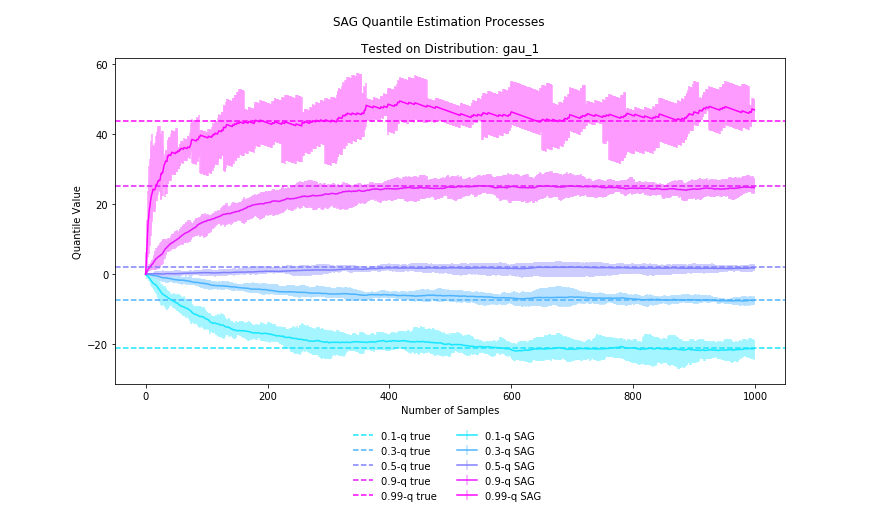
\includegraphics[width=1\columnwidth]{distro/gau_1_proc.png}
    \caption{SAG Process from \textit{gau-1} Distribution}
    \label{fig: sag_proc}
\end{figure}

\begin{figure}[H]
    \centering
	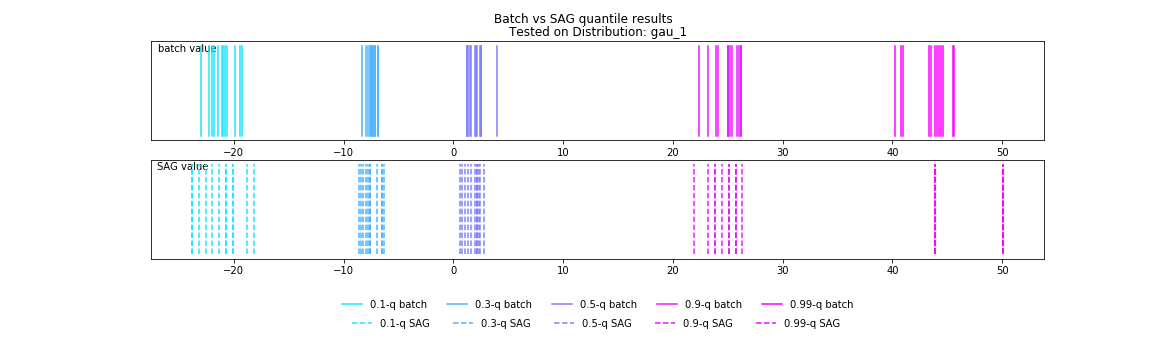
\includegraphics[width=1\columnwidth]{distro/gau_1_res.png}
    \caption{SAG Result from \textit{gau-1} Distribution}
    \label{fig: sag_res}
\end{figure}

\begin{figure}[H]
    \centering
	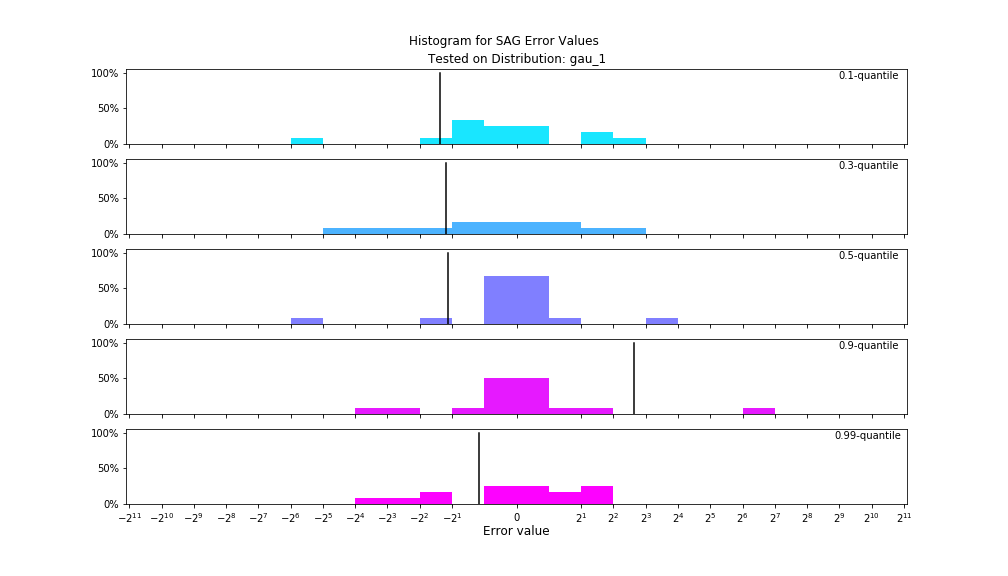
\includegraphics[width=1\columnwidth]{distro/gau_1_err.png}
    \caption{SAG Error from \textit{gau-1} Distribution}
    \label{fig: sag_err}

\end{figure}


\subsection{Smooth Functions}
\label{subsec: smooth_func}
The pinball loss function we use for the SGD quantile estimation is convex but not smooth. 
Theoretically, however, both SGD and SAG methods need smoothness for the guarantee of convergence. Although the practical experiments have shown that there is evidence of convergence in final performance, it remains a serious problem for our SGD quantile estimation methods. In this section, we present the analysis on the non-smoothness problem, followed by the potential solutions and further discussions on them.

\subsubsection{The Pinball Loss Functions}
\graphicspath{{Figures/Stepsize_adapt/Smooth_func/}{./}} 

The pinball loss function evaluates the loss from a data point $x$ for estimation of the $\tau$-quantile.

% \textbf{quote the equation of pinball loss function and it's derivative}

The fact that the pinball loss function is not differentiable at $x= 0$ is a problem for the stochastic gradient descent which uses the derivative of the objective function.

\begin{figure*}[h!]
	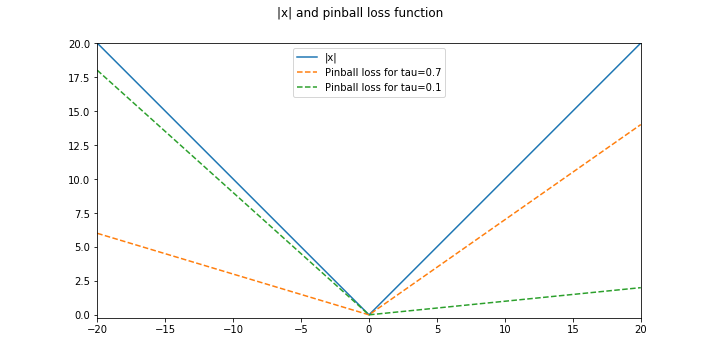
\includegraphics[width=1\columnwidth]{abs_pinball.png}
	\caption{Comparison between $|x|$ and the pinball loss function with different $\tau$ values}
\end{figure*}

The absolute value function and the pinball loss function are obviously very similar. In fact, with simple manipulation, the pinball loss function can be written in the form of absolute function as 
\begin{equation}
    l_\tau(x) = 
    \begin{cases}
        \tau \cdot |x| & {x \geq 0} \\
        (1-\tau) \cdot |x| & \text{otherwise}
    \end{cases}
\end{equation}
The pinball loss function is the combination of $|x|$ on the two parts $x<0$ and $x>0$ with different constant scale. 
If the derivative of the smooth function for $|x|$ at $x=0$ is $0$, we can also use the same approximation function respectively for the two parts of the pinball loss.
\\\\
In section \ref{subsec: smooth_sqrt} and \ref{subsec: smooth_new}, we show two approximation functions with regards to the absolute function $f = |x|$, along with the application of the approximations on the pinball loss function.

\subsubsection{Smooth function 1: a simple approxitmation}
\label{subsec: smooth_sqrt}

For $f = |x|$, a common and simple smooth approximation is $
    f = \sqrt{x^2 + \mu^2}
$.
 The convergence towards the absolute function is then proved by \citeauthor{voroninConvolutionBasedSmooth2015a}\cite{voroninConvolutionBasedSmooth2015a} that 
\begin{equation}
    ||x| - \sqrt{x^2 + \mu^2}| \leq \mu \text{  where } \mu > 0 \in \mathbb{R}
\end{equation}
\\
The smooth function application on the pinball loss function is:
\begin{equation}
    l_\tau(x) \approx 
    \begin{cases}
        \tau \cdot \sqrt{x^2 + \mu^2} & {x \geq 0} \\
        (1-\tau) \cdot \sqrt{x^2 + \mu^2} & {x < 0}
    \end{cases}
\end{equation}
and the derivative is
\begin{equation}
    l_\tau\prime(x) \approx 
    \begin{cases}
        \tau \cdot \frac{x}{\sqrt{x^2 + \mu^2}} & {x > 0} \\
        0 & {x=0} \\
        (1-\tau) \cdot \frac{x}{\sqrt{x^2 + \mu^2}} & {x<0}
    \end{cases}
\end{equation}
\subsubsection{Smooth function 2: a transcendental approximation}
\label{subsec: smooth_new}

For a better approximation accuracy, \citeauthor{bagulSMOOTHTRANSCENDENTALAPPROXIMATION2017}\cite{bagulSMOOTHTRANSCENDENTALAPPROXIMATION2017} proposes a new transcendental approximation function 
 \begin{equation}
    g(x) = x \cdot \tanh(x/\mu) \text{  where } \mu > 0 \in \mathbb{R}
 \end{equation}
which also satisfies
\begin{equation}
    ||x| - x \cdot tanh(\frac{x}{\mu})| < \mu
\end{equation}
The derivative of the approximation is
\begin{equation}
    \frac{dg(x)}{dx} = \frac{x}{\mu} \cdot sech^2 (\frac{x}{\mu}) + tanh(\frac{x}{\mu})
\end{equation}
For the pinball loss function, we now have a smooth approximation of the form:
\begin{equation}
    l_\tau(x) \approx 
    \begin{cases}
        \tau \cdot x \cdot \tanh(x/\mu) & {x\geq 0}\\
        (1-\tau) \cdot x \cdot \tanh(x/\mu) & {x < 0}
    \end{cases}
\end{equation}
and the derivative is
\begin{equation}
\label{eq:smooth_new_d}
    l_\tau\prime(x) \approx 
    \begin{cases}
        \tau \cdot \frac{x}{\mu} \cdot sech^2 (\frac{x}{\mu}) + tanh(\frac{x}{\mu}) & {x\geq 0}\\
        0 & {x=0}\\
        (1-\tau) \cdot \frac{x}{\mu} \cdot sech^2 (\frac{x}{\mu}) + tanh(\frac{x}{\mu}) & {x < 0}
    \end{cases}
\end{equation}
\subsubsection{Discussion and Conclusion}

In this part, we will compare the two alternative smooth functions in the following aspects: computer efficiency, approximation accuracy and
convexity. 
\begin{itemize}
    \item Computation efficiency: \\
    It is proved by \citeauthor{ramirezX2MostComputationally2014}\cite{ramirezX2MostComputationally2014} that $f = \sqrt{x^2 + \mu^2}$ is the most computationally efficient smooth approximation to $|x|$.
    
    On the other hand, we can see from equation \ref{eq:smooth_new_d}, the derivative for $g(x) = x \cdot \tanh(x/\mu)$ is more difficult to compute.
    \item Approximation accuracy: \\
    The following plots show intuitively how fast the two smooth functions approach to $|x|$ for $\mu = 0.01$ and $\mu = 0.001$.
    
    \begin{figure*}[h!]
        \includegraphics[width=1\columnwidth]{{mu_0.001}.png}
        \caption{Comparison between the two smooth functions when $\mu = 0.001$}
    \end{figure*}

    \begin{figure*}[h!]
        \includegraphics[width=1\columnwidth]{{mu_0.0001}.png}
        \caption{Comparison between the two smooth functions when $\mu = 0.0001$}
    \end{figure*}

    It is obvious by inspection that $ x \cdot \tanh(x/\mu)$ has a better accuracy.

    \item Convexity\\
    $f = \sqrt{x^2 + \mu^2}$ is convex and  $g(x) = x \cdot \tanh(x/\mu)$ is not.
\end{itemize}

The form of smooth function \text{does not really matter for SAG}. It is important to know the existence of Lipschitz continuous smooth function, and then the $L$ of such function must satisfy
\begin{equation}
    L \leq min(|\tau|, |1-\tau|)
\end{equation}
So that no matter which smooth function is used, we can simply take $min(|\tau|, |1-\tau|)$ to compute the step size $\alpha$ for SAG. However, we can still implement those smooth functions for SGD. Further research can be done on different smooth function implementations for SGD.

\section{Doubling and Halving SGD (DH-SGD)}
\label{sec: DH_SGD}

Although SAG has a faster convergence rate than SGD, it is clear that the fluctuation problem after convergence still exists. Is it possible that a step size adaptation of SGD can reduce the fluctuation after convergence, and at the same time have an improved convergence rate? In this section, we propose a simple algorithm called Doubling and Halving Stochastic Gradient Descent (DH-SGD), which empirically mitigates those two problems.

\subsection{Method Description}

The idea of the DH-SGD method is trivial - increase the step size if it is too big, and decrease the step size if it is too small. We choose the change of step sizes to be exponential, specifically, increasing it to double size or decrease it to half size. However, the standard on the scale of step size can be vague. 

Here we use an intuitive idea which tracks the proportion of increase and decrease updates among an interval of updates. For example, for every 200 epochs, the proportion of increase updates is $P^+$, and that of decrease update is $P^-$, we compute $P = P^+ - P^-$ as the proportional difference between the two update directions. If $P$ is too far from the ideal value $P^*$ ($\mathbb{E}(P)$ for converged quantile estimate), then it means the updates are mostly in one direction, which is likely caused when the quantile hasn't yet converged, meaning that the step size is too small. Otherwise if $P$ is close to $P^*$, it is a sign that convergence has already been reached, and reducing the step size will reduce the fluctuation. 

According to the SGD update, the current quantile estimate decrease when it sees an data point smaller than it, and increases on seeing a larger one.
This means when the quantile estimate for $\tau$-quantile has converged, the proportion of increase update $P^+_\tau$ should be the proportion of data points bigger than it, which is $1-\tau$. Similarly, we have the corresponding expectation that $P^-_\tau = \tau$.
Thus we have the ideal value for quantile probability $\tau$ defined as
\begin{equation}
    P^*_\tau = \mathbb{E}(P_\tau) = \mathbb{E}(P^+_\tau) - \mathbb{E}(P^-_\tau) = (1-\tau) - \tau = 1 - 2\tau \in (-1, 1)
\end{equation}
We use Euclidean distance to measure how close $P_\tau$ is to $P_\tau^*$. If $P_\tau \in (P^*_\tau- 0.01, P^*_\tau+ 0.01)$, it means they are close and the step size is too big. And if $P_\tau \not\in (P^*_\tau- 0.1, P^*_\tau+ 0.1)$, it means they are too far away and the step size is too small. 
The psedocode of DH-SGD is shown as algorithm~\ref{alg:DH_SGD} :

% \marginpar{THe step size scaler is different for different quantiles}
\begin{algorithm}
    \caption{DH-SGD algorithm}\label{alg:DH_SGD}
    \begin{algorithmic}[1]
        \Require{Data Stream $X$, $\tau$, $1$ unit of memory $q$, epoch check size $c$}
        \Ensure{$q$}
        % \Procedure{frugal}{$X,\tau$}            \Comment{X is the dataset}
        \State{idealProportion $P^* = 1- 2\tau$}
        \State{epochCount $ec = 0$}                       \Comment{The counter for epochs}
        \State{directionCount $dc = 0$}                   \Comment{The accumulation of directions}
        \State{scaler $s = 1$}                    \Comment{The scaler for step size}
        \State {Initialize} $q$                 \Comment{Default initialization $q_0$ = 0}
        \State{}
            \For{$x_i$ in $X$}                  \Comment{Parameter update for each input data point}
                \State{}
                \State{$ec = ec+ 1$}   
                \If{$ec$ \textit{mod} $c = 0$}            \Comment{Change scaler for every $c$ epochs}
                    \If{$\frac{dc}{c} \in (P^*-0.01, P^*+0.01) $ }               
                        \State{$s = 2s$}               \Comment{Double $s$ if the update is mostly in one direction}         
                    \Else {\textbf{if} $\frac{dc}{c} \not\in (P^*-0.1, P^*+0.1)$ \textbf{then}}  
                        \State{$s = 0.5s$}             \Comment{Halve $s$ if the update direction barely changes}
                    \EndIf
                
                \EndIf
                \State{}
                \State{\textbf{set} $\alpha_i = 1$}             \Comment{$\alpha_i$ can use other settings}
                \State{$\alpha_i = \alpha_i \cdot s$}        \Comment{Scale original step size with $s$}
                \If{$x_i > q$}                  
                    \State{$q = q + \alpha_i \tau$}
                    \State{$dc = dc + 1$}                   \Comment{Direction count $+1$ if updated upwards}
                \Else {\textbf{if} $x_i < q$ \textbf{then}}                     
                    \State{$q = q - \alpha_i (1-\tau)$}
                    \State{$dc = dc -1$}                    \Comment{Direction count $-1$ if updated downwards}

                \EndIf
            \EndFor
        \State{}
        \State \textbf{return} $q$
        % \EndProcedure
    \end{algorithmic}
\end{algorithm}

\subsection{Experiments}
\graphicspath{{Figures/Stepsize_adapt/Adaptive_stepsize/}{./}} 
\label{subsec: DB_SGD_exp}
Again we test the DH-SGD on the data stream of size 1000 of \textit{gau-1} distribution. The experiment results are shown in figure~\ref{fig: DH_SGD_proc}, \ref{fig: DH_SGD_res} and \ref{fig: DH_SGD_err}.
Interesting Observations:
\begin{enumerate}
    \item The change of step size has a very obvious improvement on convergence rate. From figure~\ref{fig: DH_SGD_proc}  we can see all the quantiles has their convergence rate at the same or faster rate compared with SGD. For example, both $0.99$ and $0.9$-q DH-SGD have a doubled step size at epoch 200, and the former reaches its convergence around epoch 900 (compared with more than 1000 in SGD) and the latter reaches convergence within 300 epochs (compared with around 600 in SGD). The other three quantiles have basically the same convergence rate.
    
    \item The fluctuation after convergence are also improved overall. All the quantiles except for the $0.1$-q DH-SGD has a denser results distribution around the batch results (figure~\ref{fig: DH_SGD_res}). However, there are also results that stand out from nearly every estimation distribution, which means the reduction of fluctuation is not consistent.
    
    \item The effect on error value is a combined result from denser distribution of accurate results and an increased number of outliers. Take the $0.99$-q DH-SGD in figure~\ref{fig: DH_SGD_err} for example, although most of the errors values are within the range ($-2^0, 2^2$), the existence of two bigger similarity values at $(-2^6, -2^5)$ and $(-2^4, -2^3)$ drag the mean error value further away from $0$. It is fair to argue the estimation error is still within the accuracy requirement range, but it is worse compared with the result in SGD, even though the $0.99$-q in SGD does not even converge. Although the fluctuation has been decreased by DH-SGD (figure~\ref{fig: DH_SGD_res}), the overall error values are also affected by only a small amount of estimations with bigger fluctuation. 
\end{enumerate}

\begin{figure}[H]
    \centering
	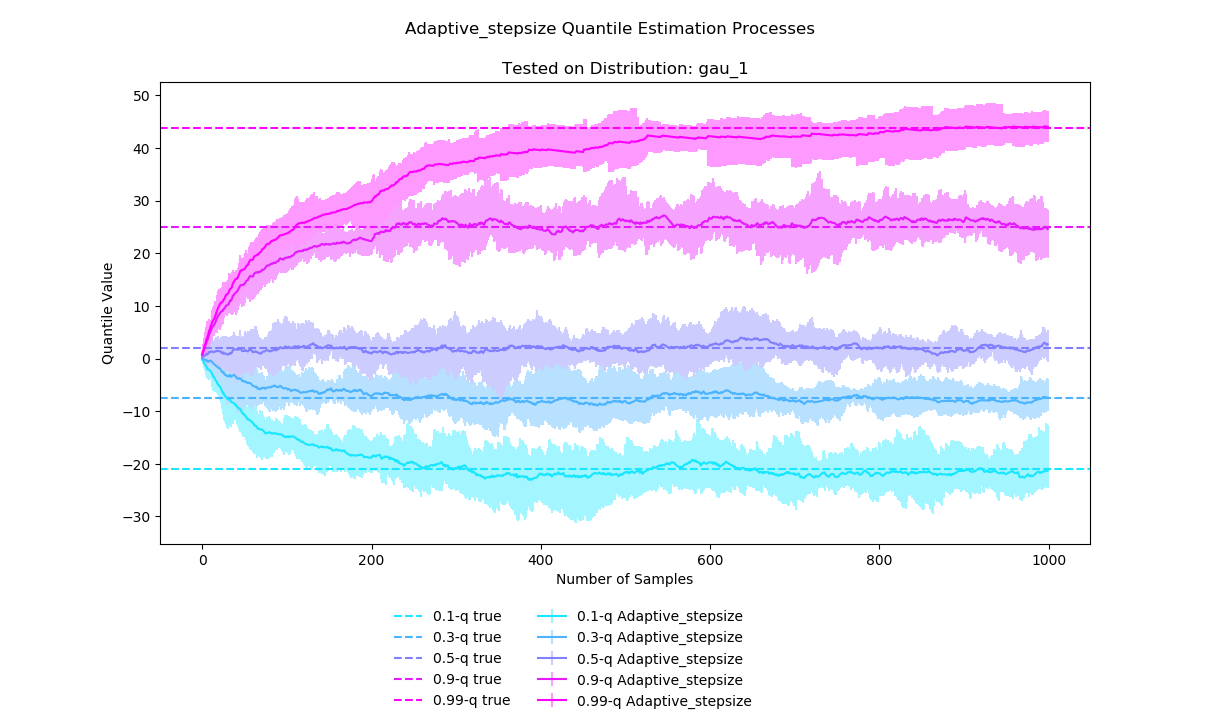
\includegraphics[width=1\columnwidth]{distro/gau_1_proc.png}
    \caption{DH-SGD Process from \textit{gau-1} Distribution}
    \label{fig: DH_SGD_proc}
\end{figure}


\begin{figure}[H]
    \centering
	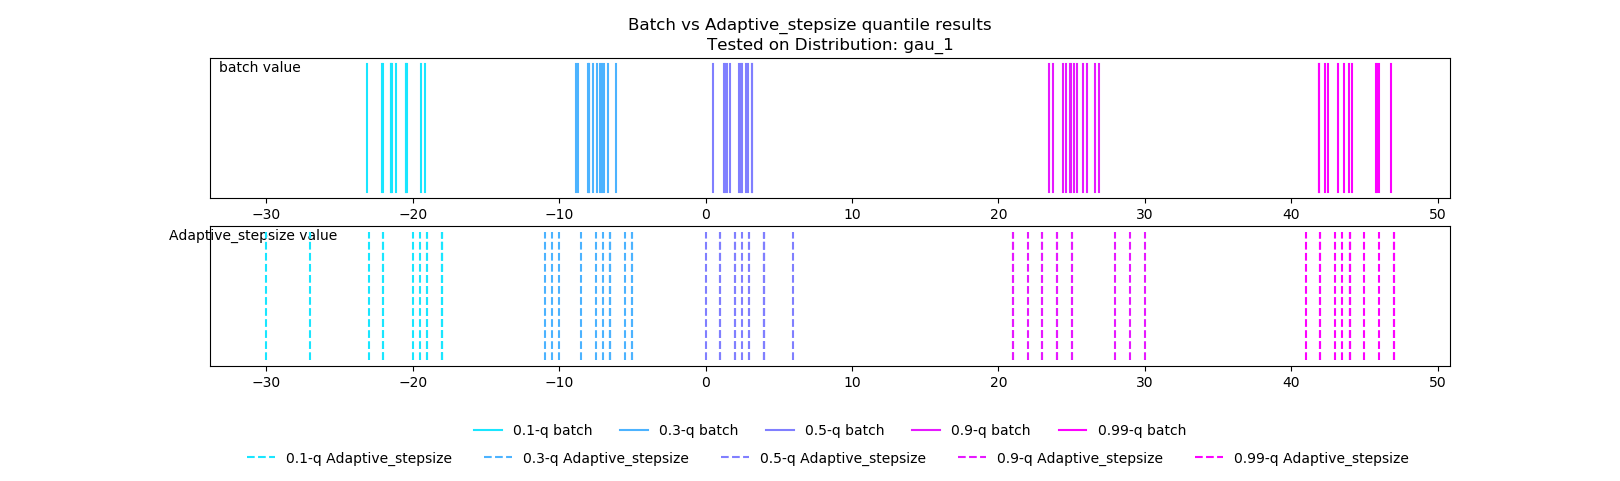
\includegraphics[width=1\columnwidth]{distro/gau_1_res.png}
    \caption{DH-SGD Results from  \textit{gau-1} Distribution}
    \label{fig: DH_SGD_res}

\end{figure}

\begin{figure}[H]
    \centering
	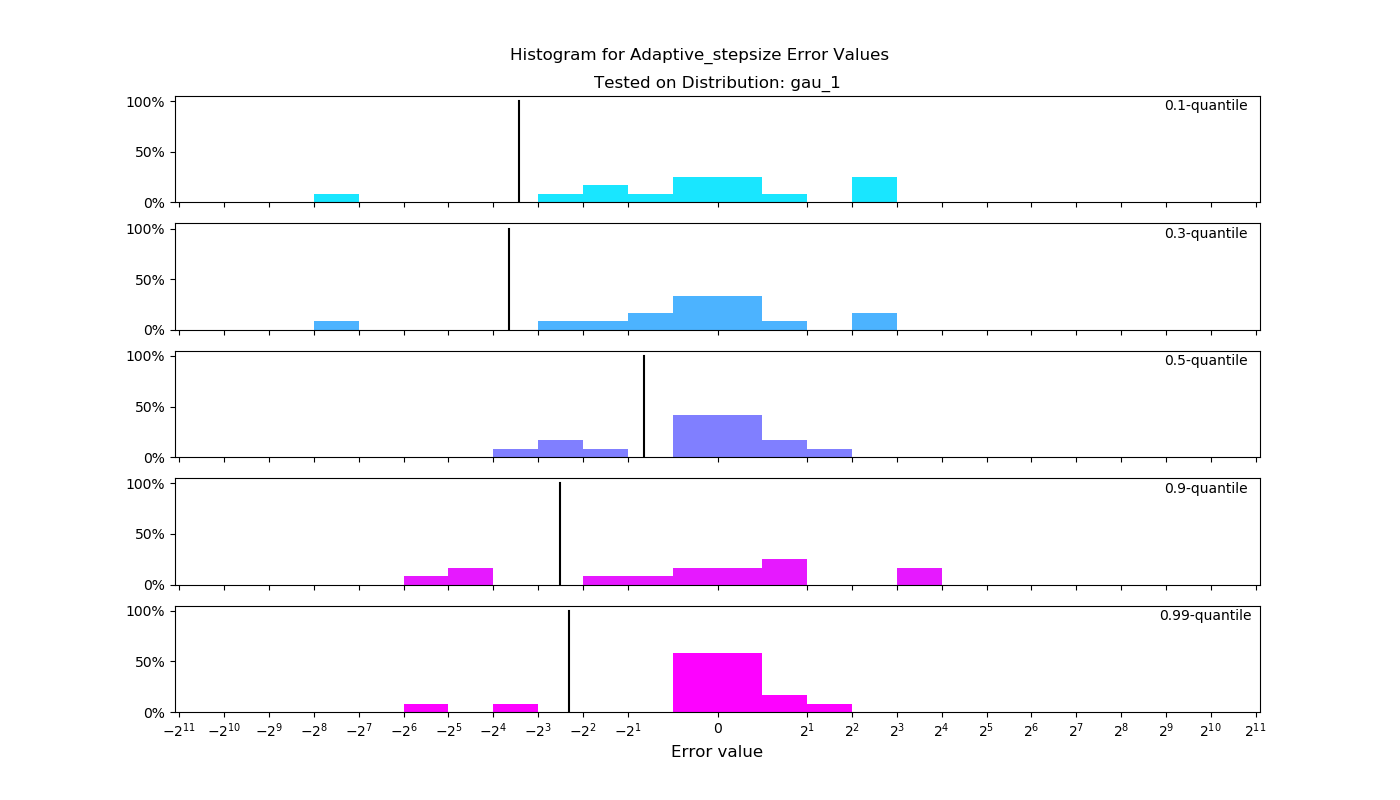
\includegraphics[width=1\columnwidth]{distro/gau_1_err.png}
    \caption{DH-SGD Error from \textit{gau-1} Distribution}
    \label{fig: DH_SGD_err}

\end{figure}

\subsection{Improvements on DH-SGD}

The small amount of estimations with fluctuation problems is a signal that the current standards for step size adaptation needs improvements. There are two potential ways for the improvements.

The first one is to change the epoch check size $c$, which determines how often to change the step size during the estimation. As the size and distribution of data stream is unknown, it is possible for the pre-defined parameter to be either too small or too big. If $c$ is small, it is more likely that the $c$ most recent updates are not a representative sample of the data, leading to the wrong change in step size. For example, if $c = 3$, it is likely that all the recent $3$ updates are in the same direction even when the estimation has converged. In this case the step size is doubled when it should have been halved. On the other hand, if $c$ is big, for example, 100000, then it takes much longer for the convergence acceleration to happen. However, we cannot know beforehand which setting is more suitable for the unknown data stream. In this situation, the choice of epoch check size is hard to be improved.

The second one is about the standards on how close is $P_\tau$ from $P_\tau^*$. The current measurement takes the same value for all $\tau \in (0,1)$, while a more accurate distance can be calculated from quantile probability $\tau$ and epoch check size $c$. Specifically, one SGD update has only two options: increase or decrease (we ignore the option to stay the same because the probability is $0$). Ideally if the quantile has already reached convergence, their probabilities are $1-\tau$ and $\tau$. The probability of having $x$ increase updates from the dataset of size $c$ is now a binomial distribution problem, where the success probability $b = 1-\tau$.
Generally, the possibility of having exactly $x$ successes with possibility $b$ from $n$ trials is:
\begin{equation}
    F(x ; n,b)=\sum_{i=0}^{ x}{\binom{n}{i}} b^{i}(1-b)^{n-i}
\end{equation}
And the distribution of the binomial probabilities are shown in figure~\ref{fig: binomial}
\begin{figure}[H]
    \centering
	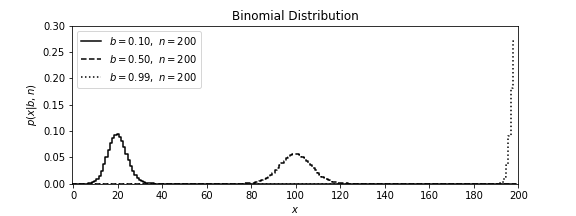
\includegraphics[width=1\columnwidth]{Binomial.png}
    \caption{DH-SGD Error from \textit{gau-1} Distribution}
    \label{fig: binomial}
\end{figure}
As shown in the plot, the distribution of the number of successful trials is different and is dependent on the success probabilities. It means the same difference $|P_\tau - P_\tau^*|$ for different $\tau$-quantiles has a different likelihood. Using this knowledge, we can improve DH-SGD by computing the distribution of the number of increases of each quantile and derive their distance standards respectively. 
%Since it is only a discussion of improvement ideas, the details of the implementation is not included here.

\section{Conclusion}
\label{sec: stepsize_adaptation_conclusion}

To sum up, SAG and DH-SGD both improve the convergence rate of SGD. SAG improves the complexity of convergence rate in theory, but in practice might slow down the convergence when the step size scaler is smaller that the SGD default step size $1$ and the convergence of SGD is already fast. The DH-SGD algorithm, on the other hand, has illustrated obvious convergence improvements on all quantiles in experiments while its convergence can not be guaranteed.

The fluctuation rate after convergence, however, is solved by neither algorithm. The step size scaler of SAG stays consistent for any updates, so the fluctuation is not improved. DH-SGD changes the step sizes regularly but does not prevent the inaccurate estimation caused by non-convergence. A potential research direction is to alleviate the fluctuation and convergence problem by a combination of SAG and DH-SGD.


\chapter{Simultaneous Multiple Quantile Estimation}
\label{ch: multi_quant}
\chapter{Conclusion}
\label{ch: conclusion}

% Problem 
% Why difficult
% Previous work
% My work
% Why important

This thesis focuses on the problem of space efficient and computationally efficient quantile estimation on data streams.
Determining quantiles helps characterize a data distribution, however due to the nature of data streams, it faces challenges in both storage and computation. The calculation of batch quantiles becomes infeasible due large amount of data, coming in at a high rate.
To solve this issue, algorithms of quantile estimation on data streams have been proposed which aim to keep a slow growing memory usage and low computational requirements for relatively accurate quantile estimates.
In this paper, we investigate the implementation of SGD method which uses constant memory and computation time per iteration for data streams of any size.
% To answer our research question, the SGD approach can be effectively applied for quantile estimation.
\\\\
We derive the SGD algorithm by implementing the SGD approach for quantile estimation. The proposed SGD algorithm is equivalent, both theoretically and empirically, to the Frugal-1U algorithm to some extent. Precisely, the algorithm equivalence analysis illustrates how the highly similar behaviours and results are affected by their difference in randomness. Since the evaluation results satisfy our tolerant requirements for equivalence, we conclude that the two algorithms are equal. This also implies that the SGD is a valid method for quantile estimation.

The convergence of SGD was empirically found to depend on several factors,
namely data distribution, data size and SGD step size settings. Data ordering was not found to have a significant impact on convergence. Of all applications, the only factor under the control of the user is the SGD setting step size. 

The newly proposed adaptation approaches of SGD step size, SAG and DH-SGD, are found to have improvement effects on convergence rate. Specifically, the SAG is theoretically proved to have a faster convergence rate while the DH-SGD convergence is tested only empirically. 
We discussed 2 smooth loss function approximations for SAG, but neither completely resolves the issue of convexity and continuity.
% Explore the extension on multi-quantile estimation. Compared two algorithms shiftQ and P2.

\section{Future work}

Step size is not the only SGD setting that affects the quantile estimation performance. As is mentioned before, other SGD settings like initialization of quantile estimates are also potentially influential factors. In the current setting of SGD, the initialization of any $\tau$-quantile ($\tau \in (0,1)$), the initialization is always $0$. The study on estimate initialization methods, for example using the first few sorted observations as starting points, is a possible direction for future work.

Another research direction is to explore more on our two current step size adaptation algorithms. Both SAG and DH-SGD are shown to have empirical acceleration effects on convergence, but they both have the unstable fluctuation problem after convergence as well as other limitation. Especially, we are concerned about the lack of convergence guarantee from DH-SGD although it provides significant improvements in some situations. It is worthwhile to consider a new algorithm that combine the idea of both SAG and DH-SGD in step size adaptation such that the convergence is guaranteed and the step size is improved.

In addition to step size adaptation, another alternative improvement direction called simultaneous multi-quantile estimation is illustrated in chapter~\ref{ch: multi_quant}. 
The shiftQ and $P^2$ algorithms introduce different ways of keeping positive distance between each adjacent quantiles at each update iteration. It is possible that some future SGD method can implement their ideas to guarantee the monotone property of a sequence of quantile estimates.

One of the ignored issue is the use of gradient descent on the non-smooth function. Theoretically, gradient descent is not applicable for the pinball loss function which is not differentiable at $0$, this application of SGD is in theory not entirely valid. However, in practice the possibility of reaching the $0$ point is $0$, and the setting of the gradient to zero at it makes sense. It is also shown in the experiment that the performance of the SGD algorithm works effectively in spite of the defective algorithm deduction. In theory, however, there is still work for the validness of SGD.


\section{Summary}
Stochastic gradient descent is a workhorse of modern machine learning methods. Here it is used to analyse quantile estimation from data streams, and is shown equivalent to a recent method from the database systems literature. We explore the empirical performance of SGD, step size adaptation approaches and two algorithms for estimation of multiple quantiles. We hope that this connection between a machine learning approach and a streaming data problem in data analysis will provide a fruitful avenue of future research.


\cleardoublepage % Empty page before the start of the next part

%------------------------------------------------
% part 2

% \ctparttext{You can put some informational part preamble text here. Illo principalmente su nos. Non message \emph{occidental} angloromanic da. Debitas effortio simplificate sia se, auxiliar summarios da que, se avantiate publicationes via. Pan in terra summarios, capital interlingua se que. Al via multo esser specimen, campo responder que da. Le usate medical addresses pro, europa origine sanctificate nos se.} % Text on the Part 2 page describing the content in Part 2

% \cleardoublepage % Empty page before the start of the next part
% \appendix
% \part{Appendix} % New part of the thesis for the appendix

%----------------------------------------------------------------------------------------
%	THESIS CONTENT - APPENDICES
%----------------------------------------------------------------------------------------

% \include{Chapters/Chapter0A} % Appendix A
%\include{Chapters/Chapter0B} % Appendix B - empty template

%----------------------------------------------------------------------------------------
%	POST-CONTENT THESIS PAGES
%----------------------------------------------------------------------------------------

% Bibliography

\label{app:bibliography} % Reference the bibliography elsewhere with \autoref{app:bibliography}

\manualmark % Work-around to have small caps also here in the headline
\markboth{\spacedlowsmallcaps{\bibname}}{\spacedlowsmallcaps{\bibname}} % Work-around to have small caps also
%\phantomsection
\refstepcounter{dummy}

\addtocontents{toc}{\protect\vspace{\beforebibskip}} % Place the bibliography slightly below the rest of the document content in the table of contents
\addcontentsline{toc}{chapter}{\tocEntry{\bibname}}

\printbibliography % Bibliography

% \cleardoublepage% Declaration

\refstepcounter{dummy}
\pdfbookmark[0]{Declaration}{declaration} % Bookmark name visible in a PDF viewer

\chapter*{Declaration} % Declaration section text

\thispagestyle{empty}

Put your declaration here.
\bigskip
 
\noindent\textit{\myLocation, \myTime}

\smallskip

\begin{flushright}
\begin{tabular}{m{5cm}}
\\ \hline
\centering\myName \\
\end{tabular}
\end{flushright}
 % Declaration


%----------------------------------------------------------------------------------------

\end{document}
